\documentclass[12pt]{article}
\usepackage[a4paper,fancysections,titlepage]{polytechnique}
\usepackage{amsmath,amssymb,bm,empheq,graphicx,hyperref,pifont,
siunitx,subcaption,upgreek,xcolor}
\usepackage[italicdiff]{physics}
\usepackage[justification=centering]{caption}
\usepackage{indentfirst}
\usepackage{subcaption}
\usepackage{graphicx}
\usepackage[section]{placeins}

\newcommand{\emptybox}{$\square$}
\newcommand{\cmark}{\ding{51}}%
\newcommand{\done}{\rlap{$\square$}{\raisebox{2pt}{\large\hspace{1pt}\cmark}}%
\hspace{-2.5pt}}

\hypersetup{colorlinks=true, urlcolor=cyan}
\newcommand{\angstrom}{\textup{\AA}}
\newcommand{\ddfrac}[2]{{\displaystyle\frac{\displaystyle #1}{\displaystyle #2}}}
\newcommand\myeq{\mathrel{\overset{\makebox[0pt]{\mbox{\normalfont\tiny\sffamily IBPx2}}}{=}}}

\title{Quantum Criticallity in Cuprate Superconductors: PRL Report}
\author{Matéo Rivera, Saleh Shamloo Ahmadi\\Supervisor: Gaël Grissonnanche}
\date{March 17, 2025}

\begin{document}
\maketitle
\tableofcontents
\newpage
\section{Introduction \& Problem Statement}

We carried out our project under the supervision of Prof. Gaël Grissonnanche in his group at \textit{Laboratoire des Solides Irradiés} (Laboratory for Irradiated Solids, LSI). 
The LSI is a joint research unit of CNRS, CEA and École polytechnique, hosted on École polytechnique's campus.
It notably hosts an electron irradiator used by researchers worldwide to add controlled disorder to materials ranging from cements in nuclear power plants to satellite photovoltaics and quantum materials.

The group's research focuses on the study of quantum materials under extreme temperature and magnetic field conditions. 
Their laboratory consists of two refrigerators that can go from room temperature to near absolute zero ($\sim 10$ millikelvin).
These refrigerators are equipped with a large superconducting magnet, 
each capable of operating at up to 14 teslas.

As our project was numerical (leveraging published experimental data),  
we didn't carry out experiments using this equipment and were supervised by Prof. Grissonnanche only. 


\subsection{Cuprates: High temperature superconductors}
\begin{figure}
    \centering
    \begin{subfigure}{0.37\textwidth}
        \centering
        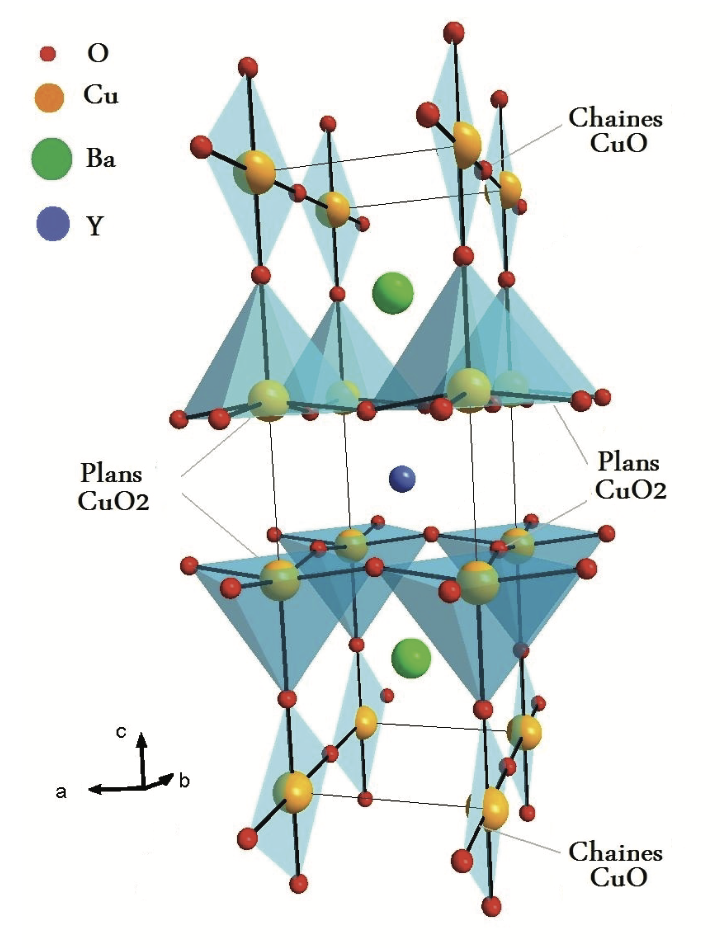
\includegraphics[width=\textwidth]{figures/cuprate_structure}
        \caption{Crystal structure of a Cuprate (YBCO)}
        \label{fig:cuprate_structure}
    \end{subfigure}\hfill
    \begin{subfigure}{0.5\textwidth}
        \centering
        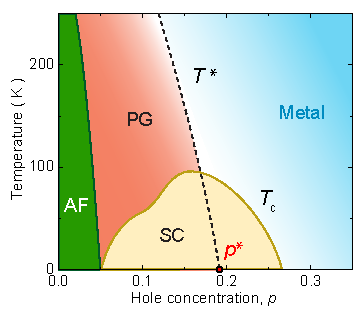
\includegraphics[width=\textwidth]{figures/phase_diagram}
        \caption{Phase diagram of cuprates}
        \label{fig:phase_diagram}
    \end{subfigure}
    \caption{Physical description of cuprates. (a) shows the provskite structure of a cuprate,
    and (b) shows the different phases of cuprates in a phase diagram. $p^*$ marks the hypothesised
    quantum critical point. AF, PG, and SC stand for Antiferromagnetic, Pseudogap, and
    Superconducting phases respectively.}
\end{figure}

Cuprates are a class of superconductors with high critical temperature that have been subject
to intense research since their discovery in 1986 because the origin of their superconductivity is not well understood. They have a general formula $XYCu_mO_n$ (where $X$ and $Y$ can be a variety of elements) and exhibit rich physical behavior, 
with a diverse phase diagram.

The crystal structure of cuprates is a perovskite structure, with a copper-oxygen plane
($\mathrm{CuO}_2$) as the main conducting layer. This structure is shown in Figure
\ref{fig:cuprate_structure}. You can think of cuprates as a stack of different conducting layers,
so the electronic properties of cuprates are mainly 2D. However, the interlayer coupling is
non-negligible, and the 3D nature of cuprates is important for their physical properties.

The phase diagram of cuprates is shown in Figure \ref{fig:phase_diagram}. The main phases of
cuprates are the antiferromagnetic (AF) phase, the metallic phase, the pseudogap (PG) phase,
the superconducting (SC) phase. 
The metallic phase itself can be split into a strange metal phase 
(with anomalous electronic scattering properties) and a normal metal phase 
(with well-described conductivity, using Fermi liquid theory).
The pseudogap phase is one of the most intriguing phases in the phase diagram, 
with many peculiarities (such as no real phase transition with the metallic phase), 
the details of which are beyond the scope of our project.
There is also a hypothesised point in the phase diagram called the quantum critical point, marked as $p^*$ in the figure.

\subsection{Origin of Cuprate Superconductivity: The Quantum Critical Point}
\begin{figure}
    \centering
    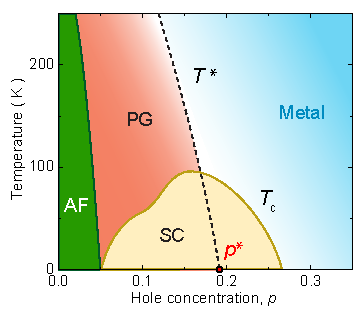
\includegraphics[width=0.5\textwidth]{figures/phase_diagram}
    \caption{Phase diagram of Cuprates. $p^*$ marks the QCP.}
    \label{fig:phase_diagram}
\end{figure}

The origin of high-temperature superconductivity in Cuprates is still the subject of intense
research and debate, but a possible explanation has to do with the Quantum Critical Point (QCP).
The QCP is a point in the phase diagram of a material where there is a phase transition at zero
temperature. This phase transition is driven by quantum effects, hence the name. In the case of
Cuprates, this is a critical doping level, usually denoted by $p_c$ or $p^*$. The actual existence
of a QCP for Cuprates is still a matter of debate and it is the subject of this project.

In their 2019 paper, Michon et al. \cite{michon2019} used secific heat measurements to
show the existence of the QCP. The effective mass of the charge carriers is expected to diverge at
the QCP, and the effective mass is proportional to $C/T$ where $C$ is the specific heat attributed
to the charge carriers and $T$ is the temperature. So, to probe the QCP, Michon et al. measured
the specific heat at very low temperatures (1 to 2 K) and extrapolated to zero temperature. More
specifically, they show
\begin{equation}
    \frac{C(T)}{T} = \gamma + \beta T^2.
\end{equation}
They found $\gamma$ peaks at the critical doping level, which is the signature of the QCP.
\begin{figure}
    \centering
    \begin{subfigure}{0.48\textwidth}
        \centering
        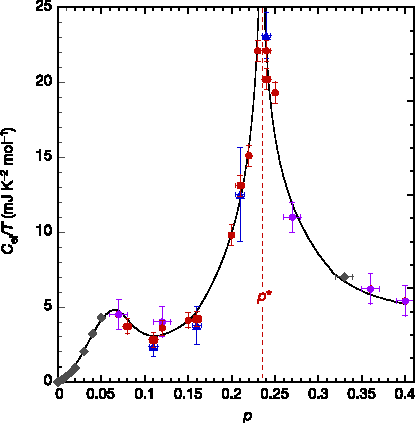
\includegraphics[width=\textwidth]{figures/michon}
        \caption{Michon et al.\cite{michon2019}}
        \label{fig:michon}
    \end{subfigure}\hfill
    \begin{subfigure}{0.48\textwidth}
        \centering
        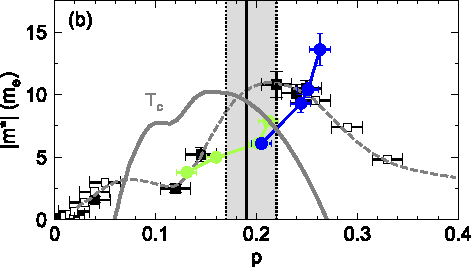
\includegraphics[width=\textwidth]{figures/legros}
        \caption{Legros et al.\cite{legros2022}}
        \label{fig:legros}
    \end{subfigure}
    \caption{Comparison of the measurements of Michon et al. Legros et al. In (a), measurements
    of Michon et al. showing a peak in $C/T$ which signifies the existence of a QCP. In (b),
    measurements of Legros et al. drawn onto the measurements from Michon et al.,
    showing no peak in the cyclotron mass.}
    \label{fig:comparison}
\end{figure}

\subsection{Evidence against the QCP: Optical Conductivity}
In their 2022 paper, Legros et al.\cite{legros2022} instead used optical conductivity to
probe the QCP. To do so, the first measured the optical conductivity of LSCO cuprates in various
fields. Then, they fitted a model for the conductivity called the Drude formula to the data. The
Drude formula is a simple classical model that has been used for a long time in condensed matter
physics to model conductivity. Next, they extracted the cyclotron mass from the parameters of the
fit. Finally, they extracted the cyclotron mass from the parameters of the fit. To do so, they
calculated the cyclotron frequency in different magnetic fields and found the mass by fitting a
linear relation between the cyclotron frequency and the magnetic field;
\begin{equation}
    \omega_c = \frac{eB}{m_c}.
\end{equation}
They argued the cyclotron mass is the same as the effective mass of the charge carriers
($m_c \sim m^*$), which can be a good or bad approximation.

At the end of all the analysis, Legros et al. found that the cyclotron mass does not peak
at the critical doping level and simply increases with doping (Figure \ref{fig:legros}). This is in contradiction with the
results of Michon et al. and suggests that there is no QCP in cuprates.

We believe, however, that their data analysis is problematic, because of the use of the Drude
formula. Eventhough the Drude formula is derived using classical physics, it is highly effective for
analysing the conductivity of materials, which emerges from the collective quantum behavior of the
electrons. But, this is only the case when the material has roughly isotropic electronic properties
.\footnote{more precisely, the Fermi surface needs to be approximately isotropic} This is not true
for cuprates, which have highly anisotropic electronic properties.\footnote{See Figure
\ref{fig:fermi_surface}. The Fermi surface is not anisotropic at all, and there is no reasonable
approximation for interpreting it in a roughly isotropic way.} Also, the effective mass of the
charge carriers is not necessarily the same as the cyclotron mass, but we only focus on the former
issue in this project.

\subsection{How to resolve the contradiction?}
In light of these contradicting conclusions, our project seeks to investigate a possible solution.
On the one hand, Michon et al.\cite{michon2019} probe criticality directly: 
that is, they look for a thermodynamic phase transition using a heat capacity measurement.

On the other hand, Legros et al.\cite{legros2022} probe it indirectly using a measurement of optical conductivity: 
$m_c$ is a parameter resulting from a fit of the experimental data. 
Thus, any results are dependent on the theoretical model chosen to fit the data.

An alternative to the Drude model used by Legros et al.\cite{legros2022} is the Chambers formula, 
derived from Boltzmann transport theory.  While the Drude model is derived for a
free electron (meaning it has isotropic transport properties), 
Boltzmann transport takes into account such anisotropy and more of the microscopic details of the
material.  This is particularly interesting for the study of cuprate high temperature
superconductors, where anisotropy is suspected to be of paramount importance.


\subsection{Goals}
During our project, we gradually set and met the following goals. In particular, we succeeded to: 
\begin{itemize}
	\item[\done] develop a tool to extract data from graphs published in the literature;
	\item[\done] reproduce the fitting results of the papers we extracted the data from;
	\item[\done] develop a tool to calculate a better model (Chambers' formula) by adapting existing code used for other experiments;
	\item[\done] analytically compare the two models (Drude and Chambers') and show that the latter reduces to the former under a 'free electron' hypothesis;
	\item[\done] validate the new numerical method by comparing calculated numerical results in the 'free electron' hypothesis with the Drude model;
	\item[\done] develop a fitting tool leveraging the new code and existing packages;
	\item[\done] qualitatively analyze (explore) the parameter space to prepare fitting;
	\item[\done] perform the fits and find the best fitting protocol on one data from one doping level.
	\item[\done] repeat the fitting on data from other doping levels.
	\item[\done] extract the effective mass from the fitting results.
	\item[\done] compare the results with the literature.
\end{itemize}
Due to a lack of time, we were not able to:
\begin{itemize}
	\item[\emptybox] do rigorous error analysis;
	\item[\emptybox] make a more complex model for lower doping levels;
\end{itemize}

\newpage
\section{Optical Conductivity}
\subsection{What is optical conductivity ?}
% Explain what it is and why we use it
The physical quantity of interest in this experiment is optical conductivity, 
the principle of which we will briefly explain.

Conductivity is often measured in static conditions: 
that is, for a constant or slowly varying applied electric fields. 
However, as for many physical systems, 
the dynamic response of the system is different from the static one. 

This dynamic response, 
that is the conductivity of a material under an applied electric field at a given frequency $\omega$, 
is precisely the optical conductivity $\sigma(\omega)$. 
Here, because we are talking about periodic excitations, this complex conductivity relates the amplitude and phase of current density to those of the applied electric field.

\sloppy{Optical conductivity $\sigma(\omega)$ is a powerful probe into the electronic properties of the
examined material,  giving a better insight than DC conductivity $\sigma(\omega=0)$ alone. 
Moreover, as is done in Legros et al., 
it is possible to apply an external magnetic field to the sample. 
This yields interesting behaviours such as Angle Dependent Magnetoresistance (ADMR) 
or the results of the experiment at hand.}

% Touch on the experimental setup
There are several experimental setups used to measure optical conductivity. 
While in principle, we can probe any frequency domain, 
we are in practice interested in the optical frequencies. 
In this case, there are two main categories of experiments that can be carried out: 
transmission and reflection. 


Legros et al.\cite{legros2022} chose a transmission setup through a thin film ($\sim 10$ nm, 10-100 layers) as their method. 
The full experimental setup is not without challenges but is not directly relevant to our study. 
However, we can note that since the electronic properties of cuprates are mainly 2D 
(owing to their peroskite structure, as explained above), 
the use of thin films is not unreasonable 
and doesn't affect the relevance of the results for bulk materials.
\subsection{What are the hypotheses of the Drude model?}
As was stated previously, Legros et al. used the Drude model to analyze their data. 
This phenomenological model is common and of great use, but it assumes that we study 'free electrons' that only periodically get scattered with a scattering rate $\Gamma$, 
which is strictly speaking false for electrons in solids, 
where they interact with a periodic lattice.

We can translate this hypothesis in the language of condensed matter physics and band structure theory (which will simplify the comparison with Chambers' formula later). 
For a single electron, due to the periodicity of the lattice, 
we can define a quasi-momentum $\vec{k}$ which is a good quantum number and defines states with given energies. 
The filling of these levels according to Pauli's principle, by ascending energy, 
allows us to define a Fermi energy and corresponding Fermi surface 
which mostly determines the conduction properties of the material and can be, 
in many cases, determined experimentally and modelled theoretically.

What makes the Drude model useful is that in many cases, 
this Fermi surface can be approximated by a sphere, which yields the dispersion relation $E(\vec{k}) = \frac{\hbar\vec{k}}{2m^*}$ 
that is formally equivalent to that of a free electron (where $m^*$ is not necessarily $m_e$). 
The Drude model assumes a unique scattering rate (independent of $\vec{k}$, because it doesn't introduce this quasi-momentum). \\

In the end, Legros et al.\cite{legros2022} and others\cite{post2021} use the two-component Drude model with normal and superconducting carriers (in the presence of a magnetic field). 
In this model, the complex optical conductivity in the left/right circular polarization basis is given by :
\begin{equation}
    \sigma_{ll/rr}(\omega) = i\epsilon_0\qty(
        \frac{\omega^2_{\mathrm{p,n}}}{\omega-\omega_c+i\Gamma}
        + \frac{\omega^2_{\mathrm{p,s}}}{\omega} - \omega(\epsilon_{\infty} - 1)),
\end{equation}
where $\omega$ is the frequency of the electromagnetic waves and the adjustable parameters are
\begin{itemize}
    \item $\omega_{\mathrm{p,n}}$ and $\omega_{\mathrm{p,s}}$: plasma frequencies of the normal and
        superconducting charge carriers,
    \item $\omega_c = \frac{eB}{m_c}$: cyclotron frequency,
    \item $\Gamma$: scattering rate,
    \item $\epsilon_{\infty}$: high-frequency dielectric constant.
\end{itemize}
Left handed circular polarization is given by a negative omega and right handed by a positive omega.

As stated in Legros et al. and other sources, 
the high-frequency dielectric constant does not greatly improve the quality of the fit and its results, so it is set to 1.
Additionally, we can see here that in this model, the superconducting carriers only contribute to the imaginary part of $\sigma$. 
This ended up being relevant to inform our fitting choices in the end.



\subsection{Boltzmann Transport and Chambers Formula for Optical Conductivity}
The Boltzmann transport equation is a semi-classical model of flow. 
In the context of band structure theory reminded earlier, 
and considering that the pseudo-momentum defined above applies to $N\gg 1$ actual particles (hence 'semi-classical'), 
it is closely related to the Gibbs-Liouville theorem in variational mechanics. 

This point can convince us that this approach gives a more detailed model of the electronic properties of a material, 
since it accounts for the trajectories of the electrons in phase space. 
Chambers' formula thus contains a lot more information about the electronic structure
of the material, 
which can show more subtleties in its physical description.

Using the equation, with a few reasonable assumptions, 
one can derive the Chambers formula for conductivity. 
The formula is usually applied for DC conductivity ($\sigma(\omega=0)$), 
but it can be generalized for optical conductivity too (see appendix \ref{sec:chambers}).
This model has been used successfully in the past to study the behavior of cuprates 
and make predictions about their physical properties\cite{grissonnanche2021}, 
justifying its use here.

According to the Chambers formula for optical conductivity, 
the conductivity tensor in the cartesian basis is then given by :
\begin{equation}
	\sigma_{ab} = \frac{2e^2}{(2\pi)^d\hbar}\int_{\mathrm{FS}}\dd{\vb{k}}\hat{v}_a(\vb{k})
        \int_0^{\infty}\dd{t}v_b(\vb{k}(t))\exp{i\omega t
        - \int_0^t \frac{\mathop{dt'}}{\tau(\vb{k}(t'))}}
\end{equation}
where $\mathrm{FS}$ is the Fermi surface, $d$ is the number of dimensions of the system, $\vb{k}$ is the
wavevector, $\omega$ is the frequency of the electromagnetic waves, $v_b$ is the veclocity of the
charge carriers in the $b$ direction, $\hat{v}_a\equiv v_a/\abs{\vb{v}}$, and $\tau$ is the
relaxation time (inverse of the scattering rate). 

We can have an intuitive understanding of this formula. 
First, as we see here, we are only interested in the electrons that live on (or near, strictly speaking when at nonzero temperature) the Fermi surface as defined previously. 
Indeed, it is possible to show, as was mentioned above, that only they will meaningfully contribute to conduction. 
For any starting point $\vb{k}$ on the Fermi surface (first integral) with a given associated velocity in the $a$ component, 
we are interested the electron's velocity in the $b$ component along its trajectory (parametrised by $t$,  which can be time). 
The exponential terms account for the influence of the varying electrical field and the scattering rate of electron (that is not uniform in phase space). 
The magnetic field appears implicitly in the movement equations that define $\b{k}(t)$.

Thus, the formula reflects how, on average, electrons move in the $b$ direction when initially excited in the $a$ direction.


In order to evaluate the integral, we should then couple it with :
\begin{enumerate}
    \item a movement equation;
    \item a model for the scattering rate;
    \item the shape of the Fermi surface.
\end{enumerate}

In the following, 
we explain in more detail the different components and the methods of evaluating this formula.

\subsubsection{Movement Equation}
Since we are only interested in the first order response of the system to an electric field, we
can solve the movement equation with only a magnetic field. That is,
\begin{empheq}[left=\empheqlbrace]{align}
    \hbar\dv{\vb{k}}{t} &= e\vb{v}\times\vb{B}, \\
    \vb{v} &= \frac{1}{\hbar}\grad_{\vb{k}}\varepsilon(\vb{k}),
\end{empheq}
Where $\varepsilon$ is the energy of the charge carriers. The movement equation can be solved
numerically for a discretization of the Fermi surface (since the Chambers formula integral is
evaluated over the Fermi surface).

Here, note that the magnetic field $\vb{B}$ is always pointed along the $z$ direction for the data
we examined. However, our methods allow any direction for the magnetic field too.

\subsubsection{Scattering Rate}
Following Grissonnanche et al.\cite{grissonnanche2021}, we used a simple model for the scattering
rate, respecting the symmetry of the system. It is given by
\begin{equation}
    \frac{1}{\tau(\vb{k})} = \Gamma(\vb{k}) = \Gamma_0 + \Gamma_k\abs{\cos(2\varphi)}^\nu,
\end{equation}
where $\varphi$ is the angle between the wavevector and the $k_x$ axis and $\Gamma_0$, $\Gamma_k$,
and $\nu$ are adjustable parameters.

\subsubsection{Fermi Surface}
For the shape of the Fermi surface, we used a simple 3D tight-binding model for the Body centered
tetragonal crystal structure of LSCO, given by
\begin{equation}
\begin{aligned}
    \varepsilon(\vb{k}) = &-\mu - 2t(\cos(k_x a) + \cos(k_y a)) \\
        &- 4t'\cos(k_x a)\cos(k_y a) - 2t''(\cos(2k_x a) + \cos(2k_y a)) \\
        &- 2t_z\cos(k_x a / 2)\cos(k_y a / 2)\cos(k_z c / 2)[\cos(k_x a) - \cos(k_y a)]^2,
\end{aligned}
\end{equation}
where $\mu$ is the chemical potential, $t$, $t'$, and $t''$ are the first, second, and third
nearest-neighbor hopping parameters, $t_z$ is the interlayer hopping parameter,
$a=3.75\angstrom$ is the in-plane lattice constant, and $c/2=6.6\angstrom$ is the
$\mathrm{CuO_2}$ layer spacing. These parameters are tabulated and, for the considered samples,
can be fitted to experimental methods with good accuracy. 


\newpage
\section{Codes and tools developed}
In the following, all conductivities are expressed in $mS.cm^{-1}$
\subsection{Plot digitization}
Once we understood well the disadvantages the Drude model had, 
and the potential benefits of using Chambers' formula instead, 
we needed to get access to the experimental data in order to 
first reproduce the literature's Drude modelling and 
second run our own fits using Chambers' formula.\\

Since the raw data of Legros et al. and Post et al. is not publicly available neither in the articles nor in supplemental data files, 
we digitized it from their papers using a custom script extracting the data from SVG exports of the figures. 

Digital files of papers contain vector graphics, 
which explicitly encode graphs as points and paths with given coordinates to draw lines. 
A difficulty lies in matching what is visually one curve on a given graph to the associated points in the file structure definition 
(this can depend greatly on the program and version that were used to generate the plot). 
Once the file structure is analyzed and understood, 
we can extract the data points from the plot by reading the path data and using some reference points to set the scale.
This is a direct and semi-automatic way to do plot digitization.
 
When compared to the more traditional hand-extraction where one has to manually click on different points of the graph, 
this allows us to avoid added errors through the digitization process 
and to streamline the data extraction, extracting many curves at once.

\subsection{From ADMR to optical conductivity}

\newpage
\section{Results}
\subsection{Chambers Formula vs Drude Formula}
\begin{figure}
    \centering
    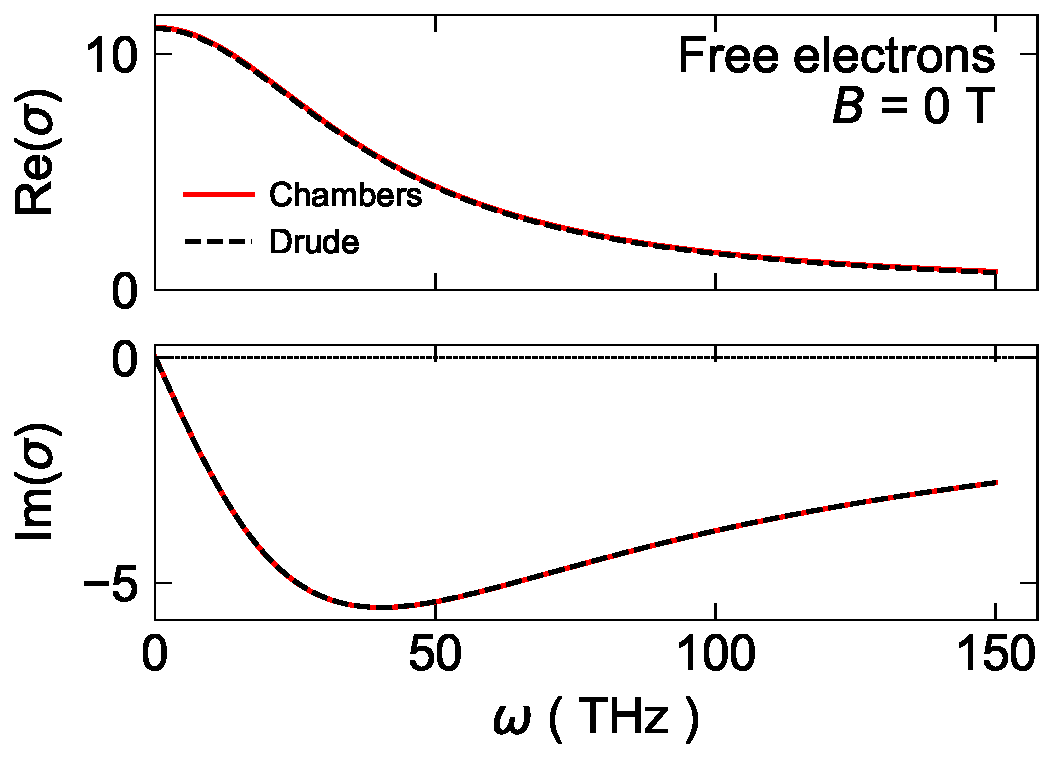
\includegraphics[width=0.7\textwidth]{figures/free_electrons}
    \caption{Agreement of the Drude and Chambers models for free electrons.}
    \label{fig:free_electrons}
\end{figure}

As we explained above, %and derived in appendix, 
the Drude model assumes that the system has particular ``free electron'' transport properties. 
This is merely a special case for the Chambers formula, 
and under these assumptions, 
both models are analytically fully equivalent (see appendix \ref{sec:equivalence}).

To make sure our numerical implementation of the new model makes sense, 
we can use this result as a form of validation of our code, on a known case. 
We compared the output of our implementation of Chambers' model in the case of free electrons to the Drude model. 
Figure \ref{fig:free_electrons} shows how the numerical model and the Drude explicit formula agree in this case.

This successful validation test gave us confidence in the soundness of our implementation for further use, 
however this test is not foolproof and we also double-checked the code itself.
\subsection{Reproduction of the Drude fits}
We could reproduce most of the results of Legros et al. (Figure \ref{fig:drude_fit_good}).
However, no matter how much we fine-tuned the fitting procedure, we could not produce fits looking
as good as theirs for some of the plots (Figure \ref{fig:drude_fit_bad}). So, we tried fitting the
real part and the imaginary part of the optical conductivity separately, and we could produce
similar-looking fits. Extracting the parameters from these fits and comparing them to the parameters
extracted from the fits of Legros et al., we found that the parameters were consistent. This leads
us to believe this is indeed what Legros et al. did in their analysis (although they did not mention
it in their paper).

Fitting the real and imaginary parts separately is not ``correct'' in some sense, but since the
imaginary part of the optical conductivity is dominated by a superconducting singularity, fitting
it separately can be a reasonable choice. This line of reasoning breaks down when there is not a
large singularity due to superconductivity, but most of these cases are well-fitted. Although, there
does exist a few cases with little superconductivity, but bad fits with simultaniously fitting the real
and imaginary parts of the optical conductivity.

To conclude, the fitting procedure of Legros et al. is badly documented and we cannot be completely
sure of their method. However, we could reproduce their results by fitting the real and imaginary
parts of the optical conductivity separately. This might be used as another objection to this paper,
but since we lack their full parameter output and details about their fitting procedure, we do not
assert that they definitly did this to ``fix'' their fits.

\begin{figure}
    \centering
    \begin{subfigure}{0.49\textwidth}
        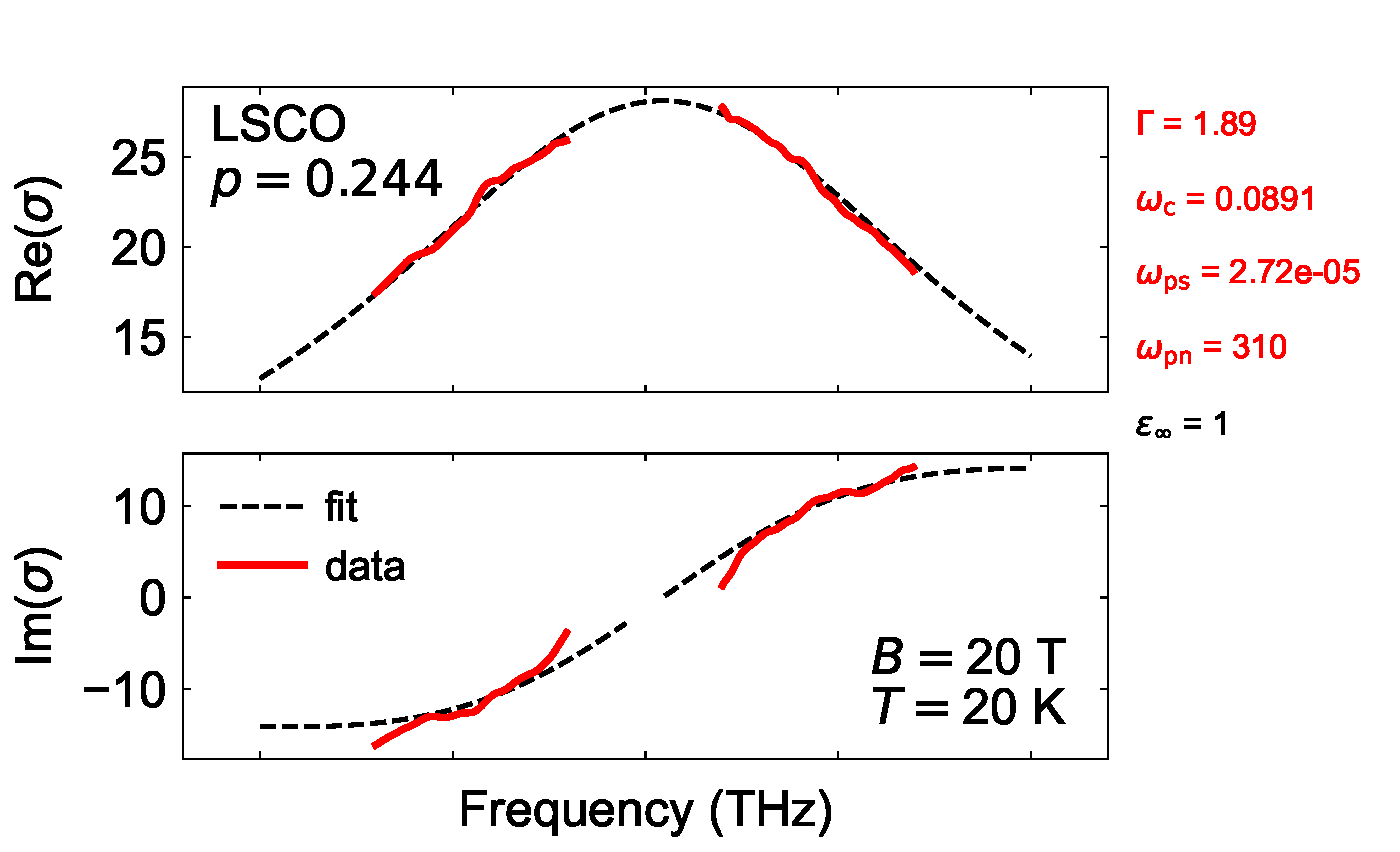
\includegraphics[width=\textwidth]{figures/drude_fit_good.pdf}
        \caption{Good fit}
        \label{fig:drude_fit_good}
    \end{subfigure}
    \begin{subfigure}{0.5\textwidth}
        \centering
        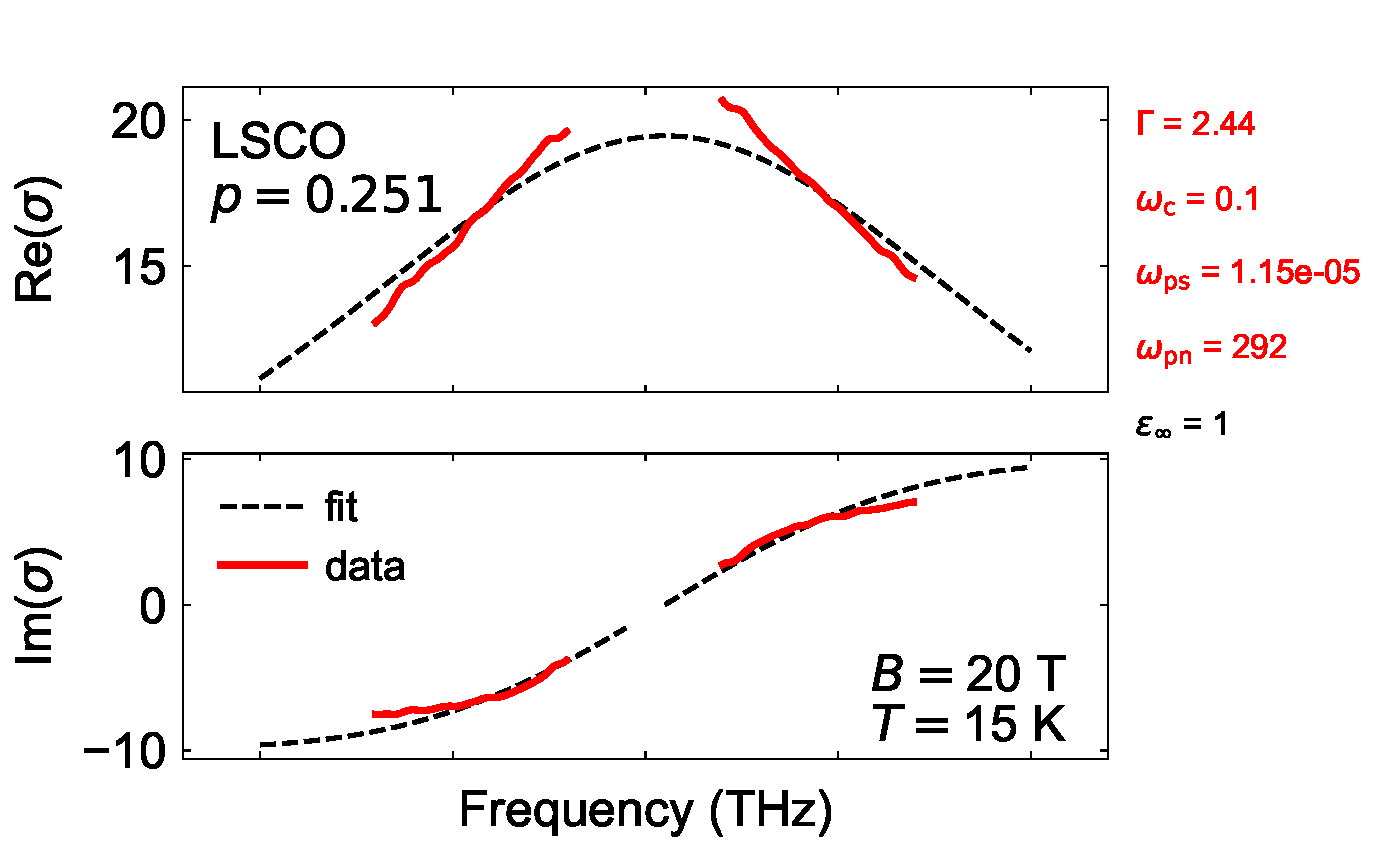
\includegraphics[width=\textwidth]{figures/drude_fit_bad.pdf}
        \caption{Bad fit}
        \label{fig:drude_fit_bad}
    \end{subfigure}
    \begin{subfigure}{0.49\textwidth}
        \centering
        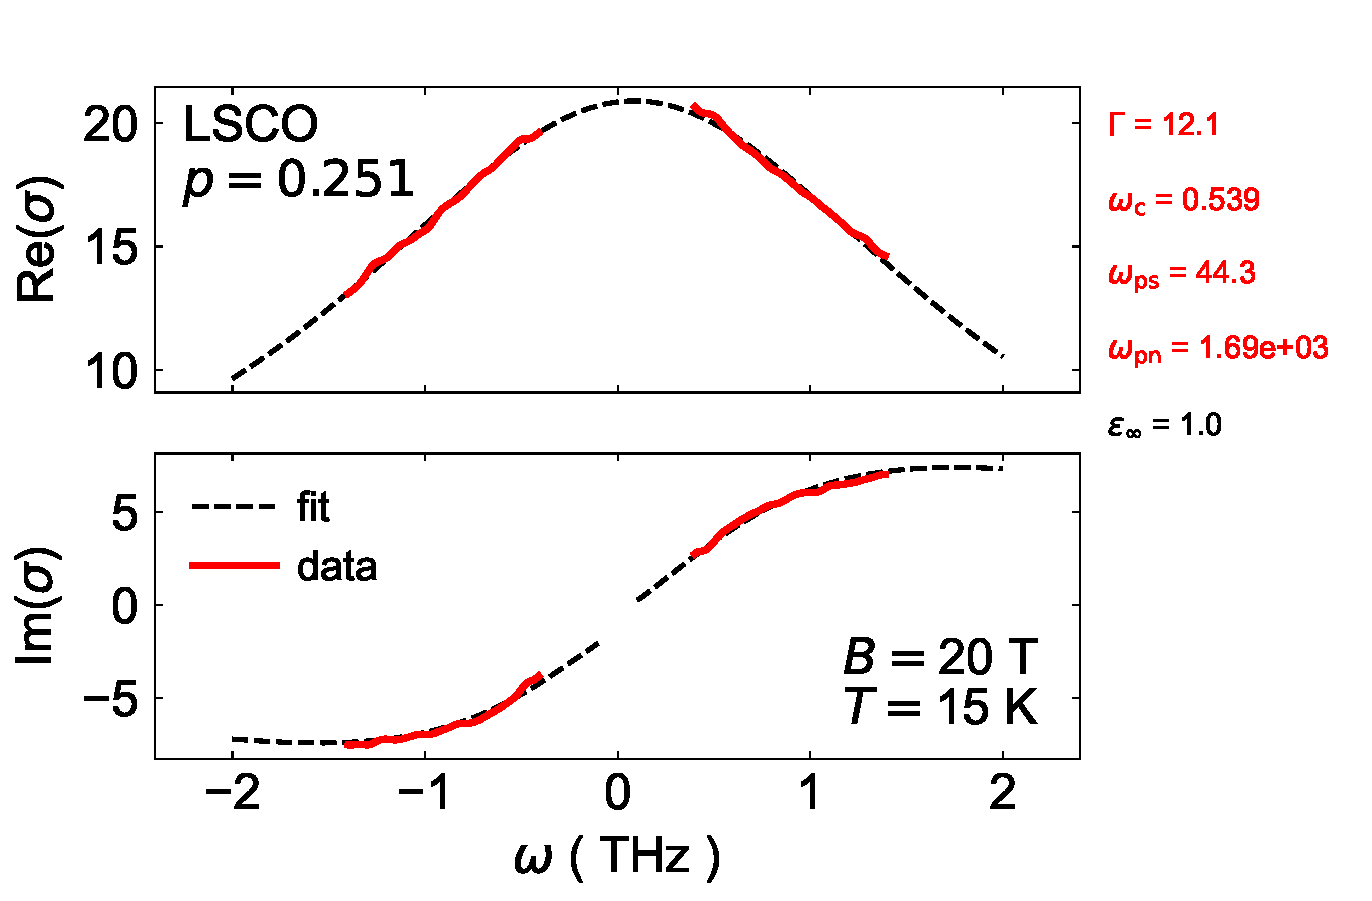
\includegraphics[width=\textwidth]{figures/drude_fit_fixed.pdf}
        \caption{Fixed fit}
        \label{fig:drude_fit_bad}
    \end{subfigure}
    \caption{(a): A good fit while fitting the real and imaginary parts of the optical conductivity
    simultaneously. (b): A bad fit while fitting the real and imaginary parts of the optical
    conductivity simultaneously. (c): A fit fixed by fitting the real and imaginary parts of the
    optical conductivity separately.}
\end{figure}

%%% We can show the reproduction of Post et al. too maybe ?
We also used data from Post et al. which we were able to reproduce quite well. 
In this case, we had no particular issues during the fitting process except for a few extraneous points. 
We were able to fit the data and recreate their plots that extract a field dependence for the $\omega_{p,n}$, $\omega_c$, and $\Gamma$ parameters of the Drude model.

For $\omega_{p,n}$ and $\Gamma$, this is something that, in principle we wouldn't want to find in the result using Chambers' formula : 
indeed, the scattering and the plasma frequency of the charge carriers should, 
in principle, not depend on $B$.

\begin{figure}
\centering
\begin{subfigure}{0.45\textwidth}
    \includegraphics[width=\textwidth]{example-image}
    \caption{Our plot}
    \label{fig:gamma_extraction_ours}
\end{subfigure}
\hfill
\begin{subfigure}{0.45\textwidth}
    \includegraphics[width=\textwidth]{example-image}
    \caption{Their plot}
    \label{fig:gamma_extraction_theirs}
\end{subfigure}
        
\caption{Reproduction of Post et al. data analysis and extraction of isotropic Drude scattering $\Gamma$ as a function of applied field $B$}
\label{fig:reproduction_post}
\end{figure}

\subsection{Optical Conductivity and Anisotropic Properties}

\begin{figure}
    \centering
    \begin{subfigure}{0.495\textwidth}
        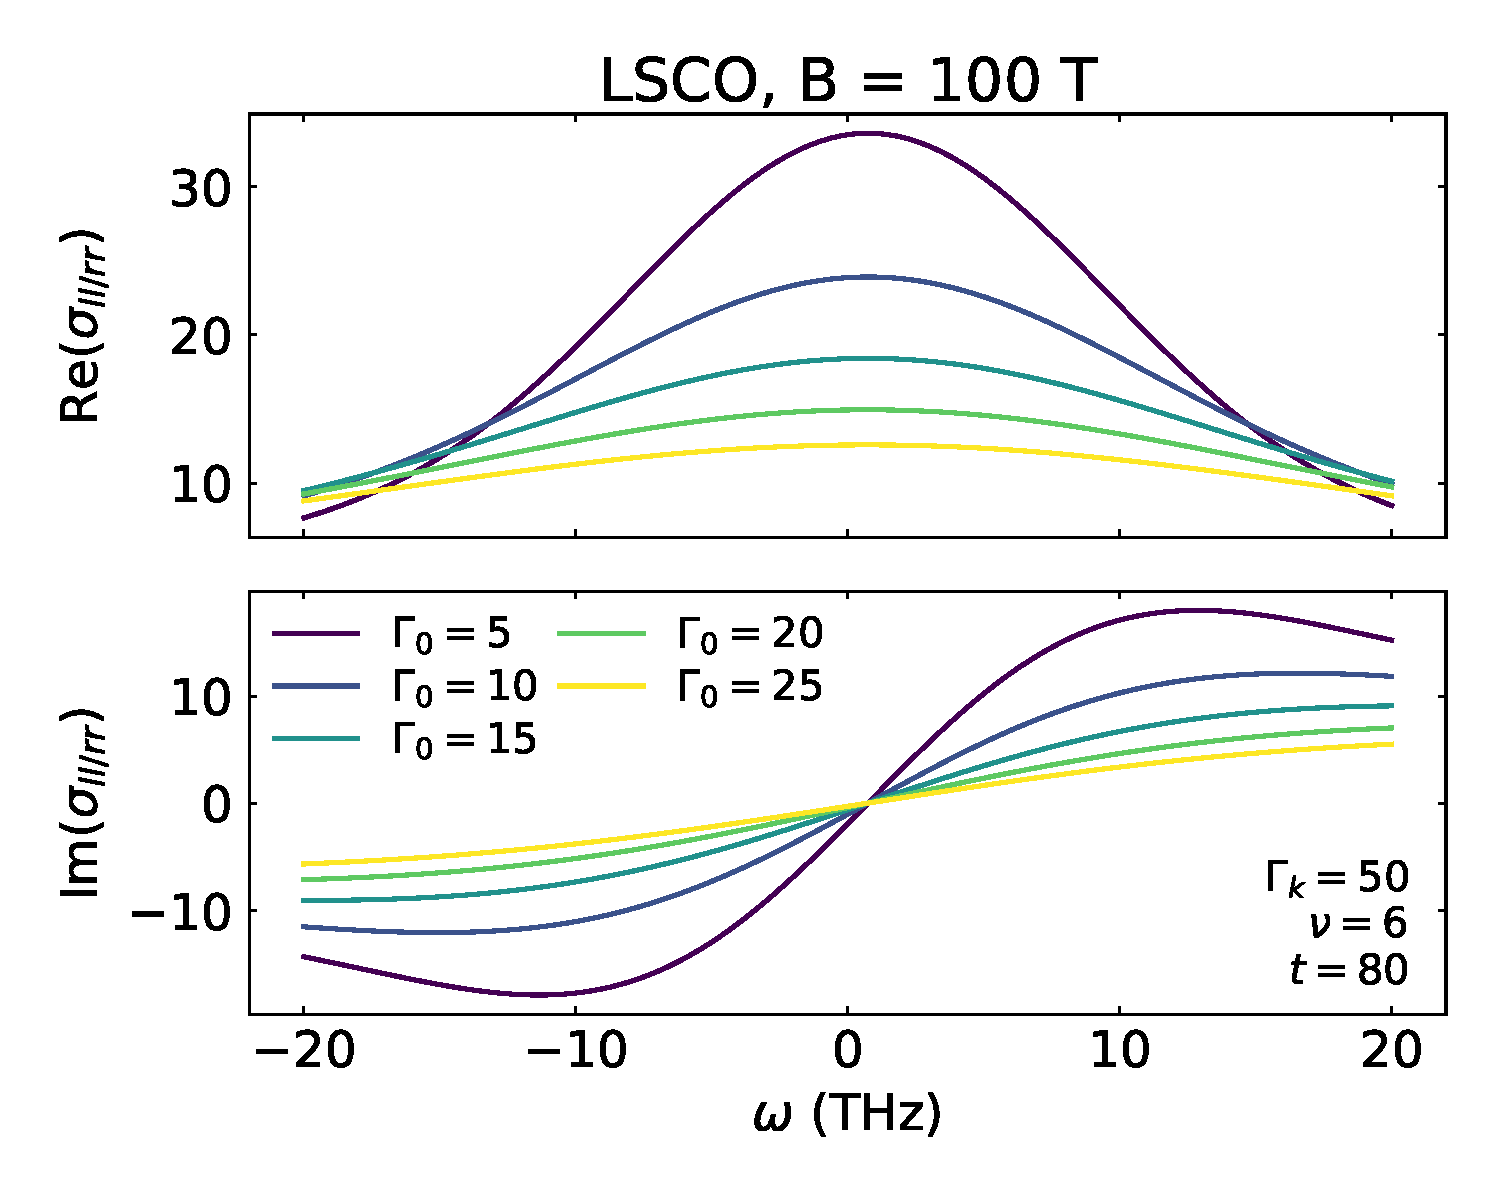
\includegraphics[width=\textwidth]{figures/vary_gamma_0}
        \caption{Varying the isotropic scattering rate}
        \label{fig:vary_gamma_0}
    \end{subfigure}
    \begin{subfigure}{0.495\textwidth}
        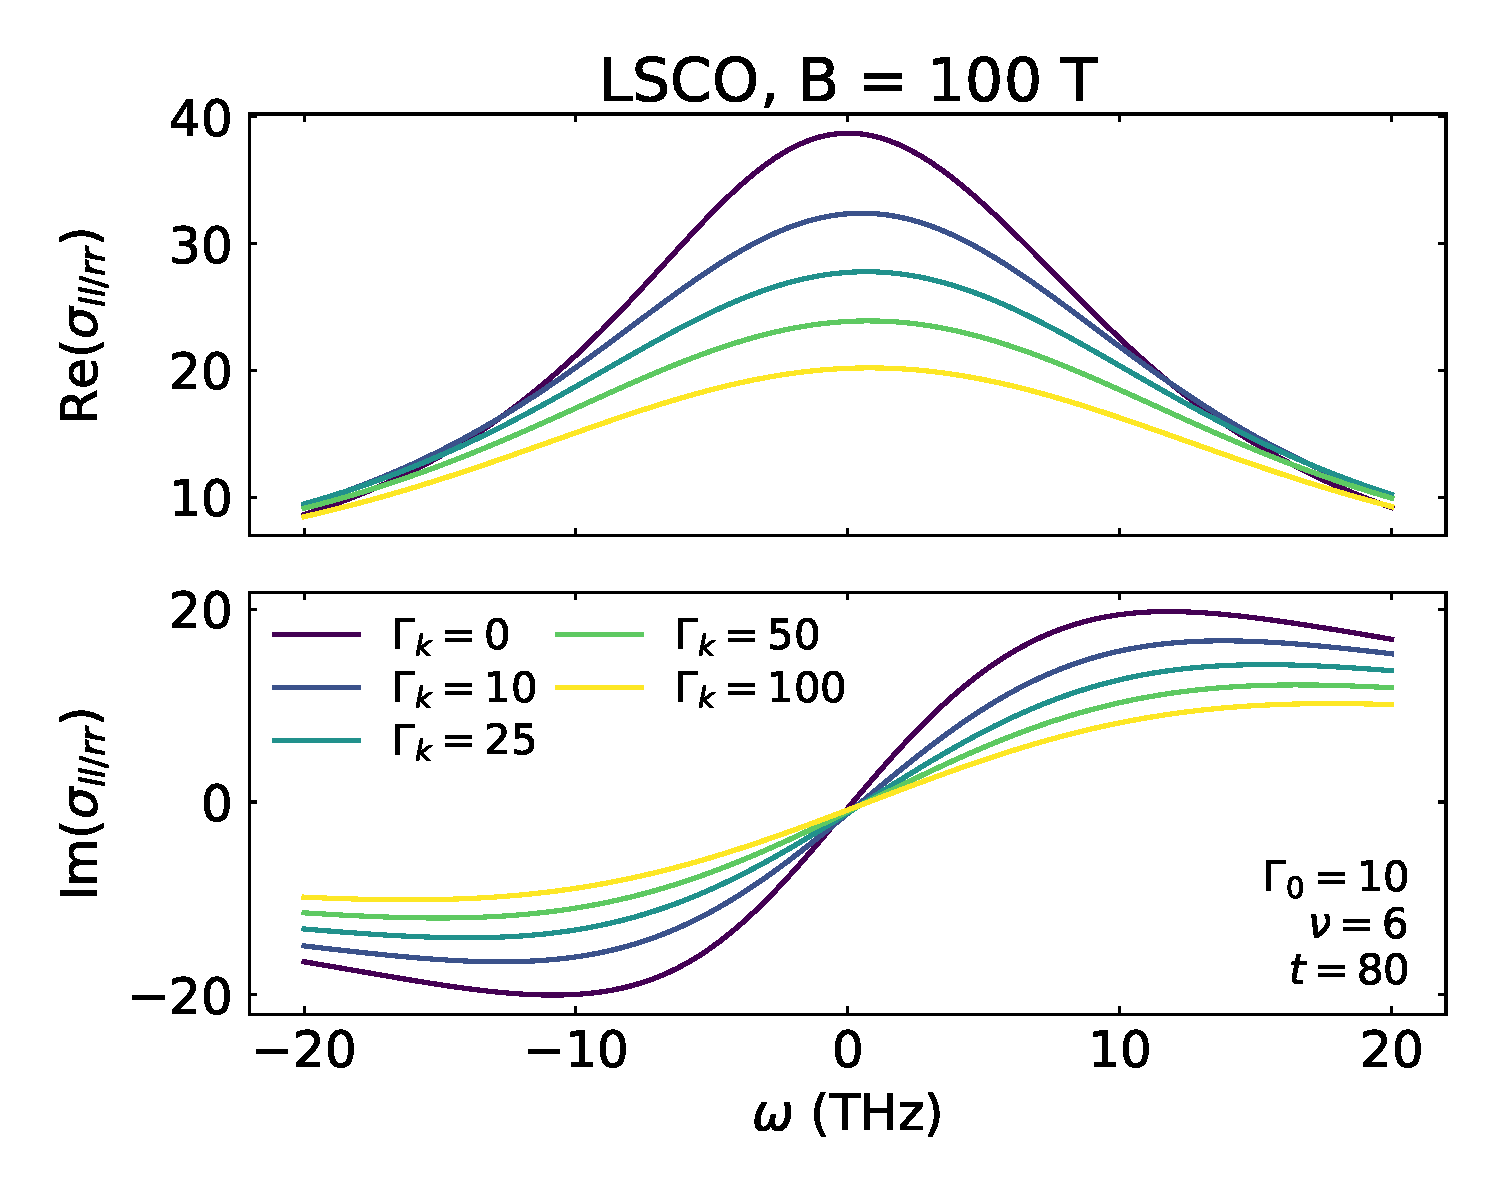
\includegraphics[width=\textwidth]{figures/vary_gamma_k}
        \caption{Varying the anisotropic scattering coefficient}
        \label{fig:vary_gamma_k}
    \end{subfigure}
    \begin{subfigure}{0.495\textwidth}
        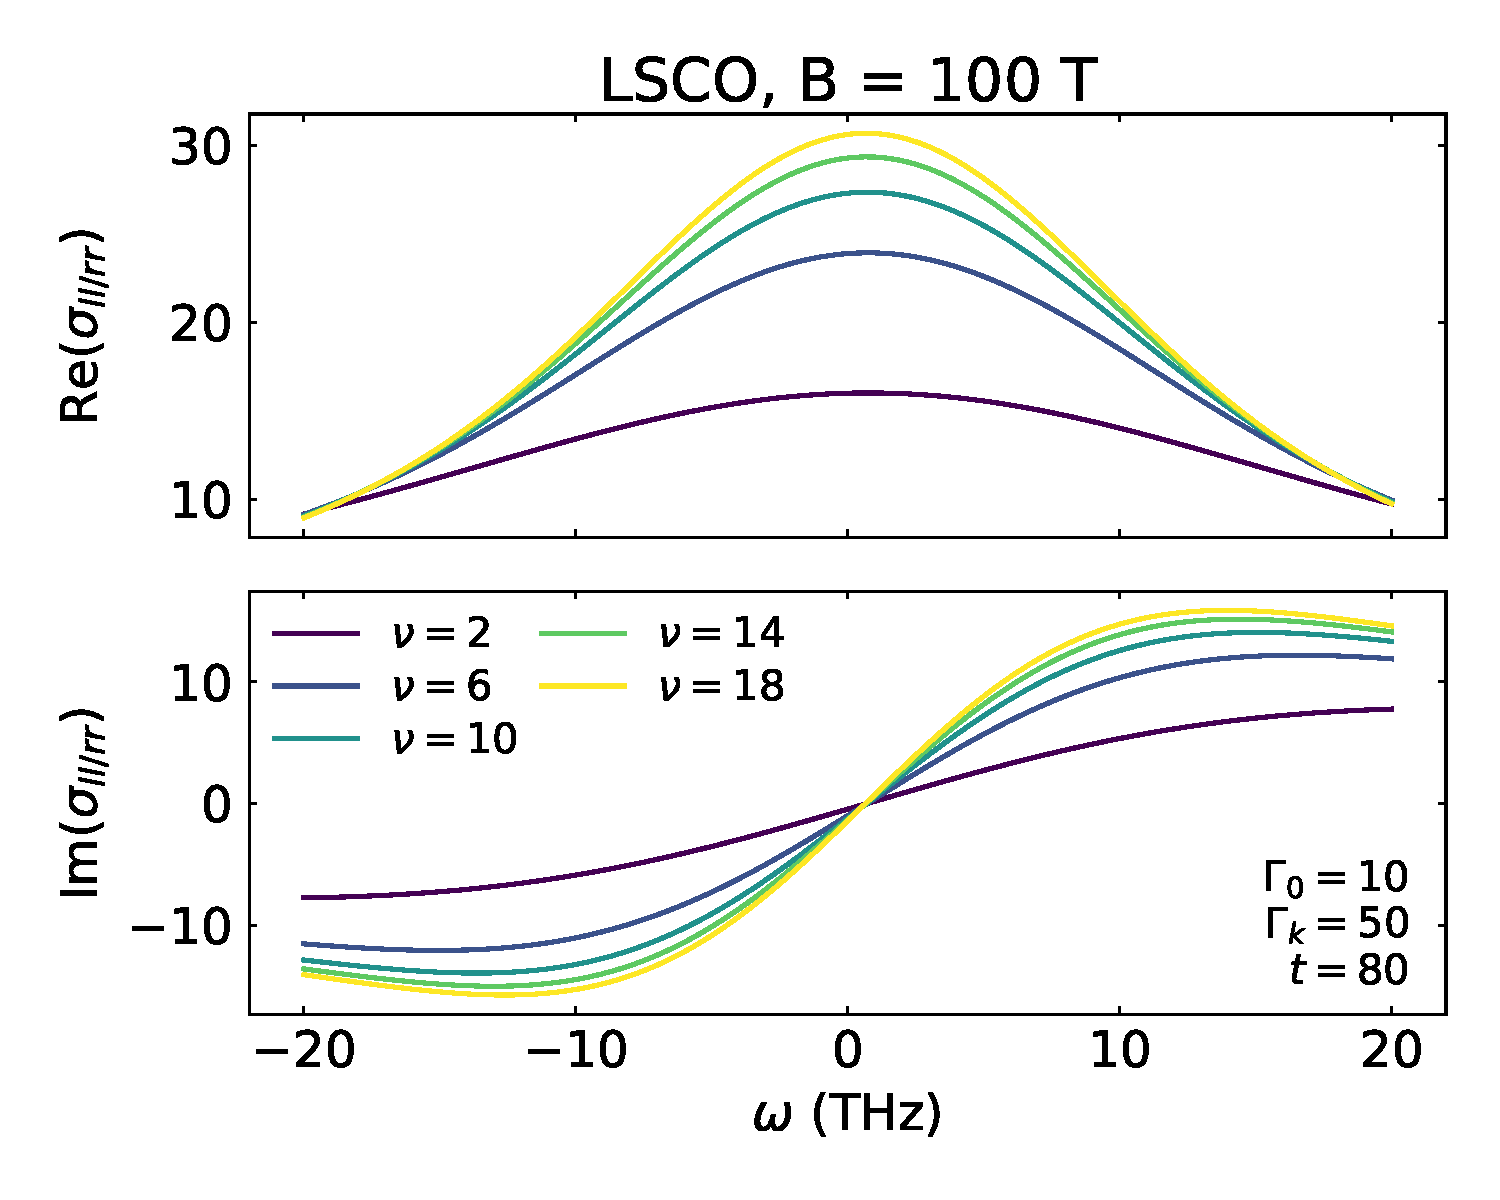
\includegraphics[width=\textwidth]{figures/vary_power}
        \caption{Varying the anisotropic scattering exponent}
        \label{fig:vary_power}
    \end{subfigure}
    \begin{subfigure}{0.495\textwidth}
        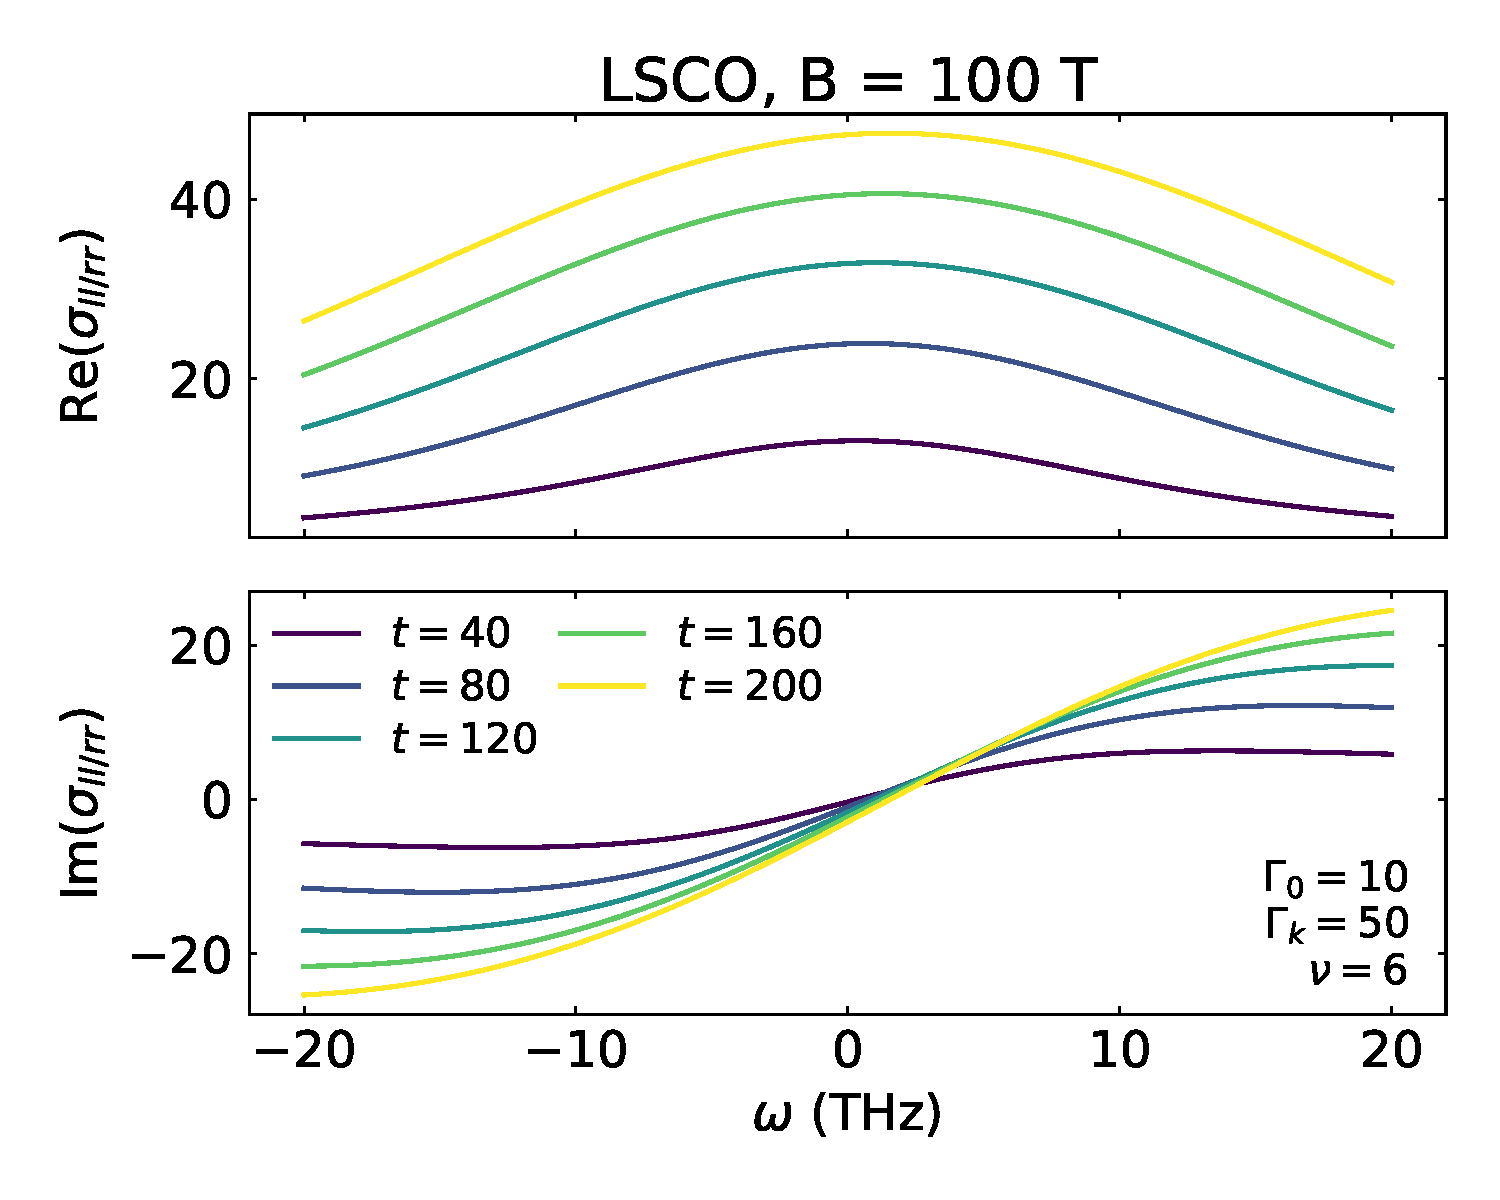
\includegraphics[width=\textwidth]{figures/vary_energy_scale}
        \caption{Varying the energy scale}
        \label{fig:vary_energy_scale}
    \end{subfigure}
    \caption{Effect of varying different model parameters}
    \label{fig:vary_parameters}
\end{figure}

\begin{figure}
    \centering
    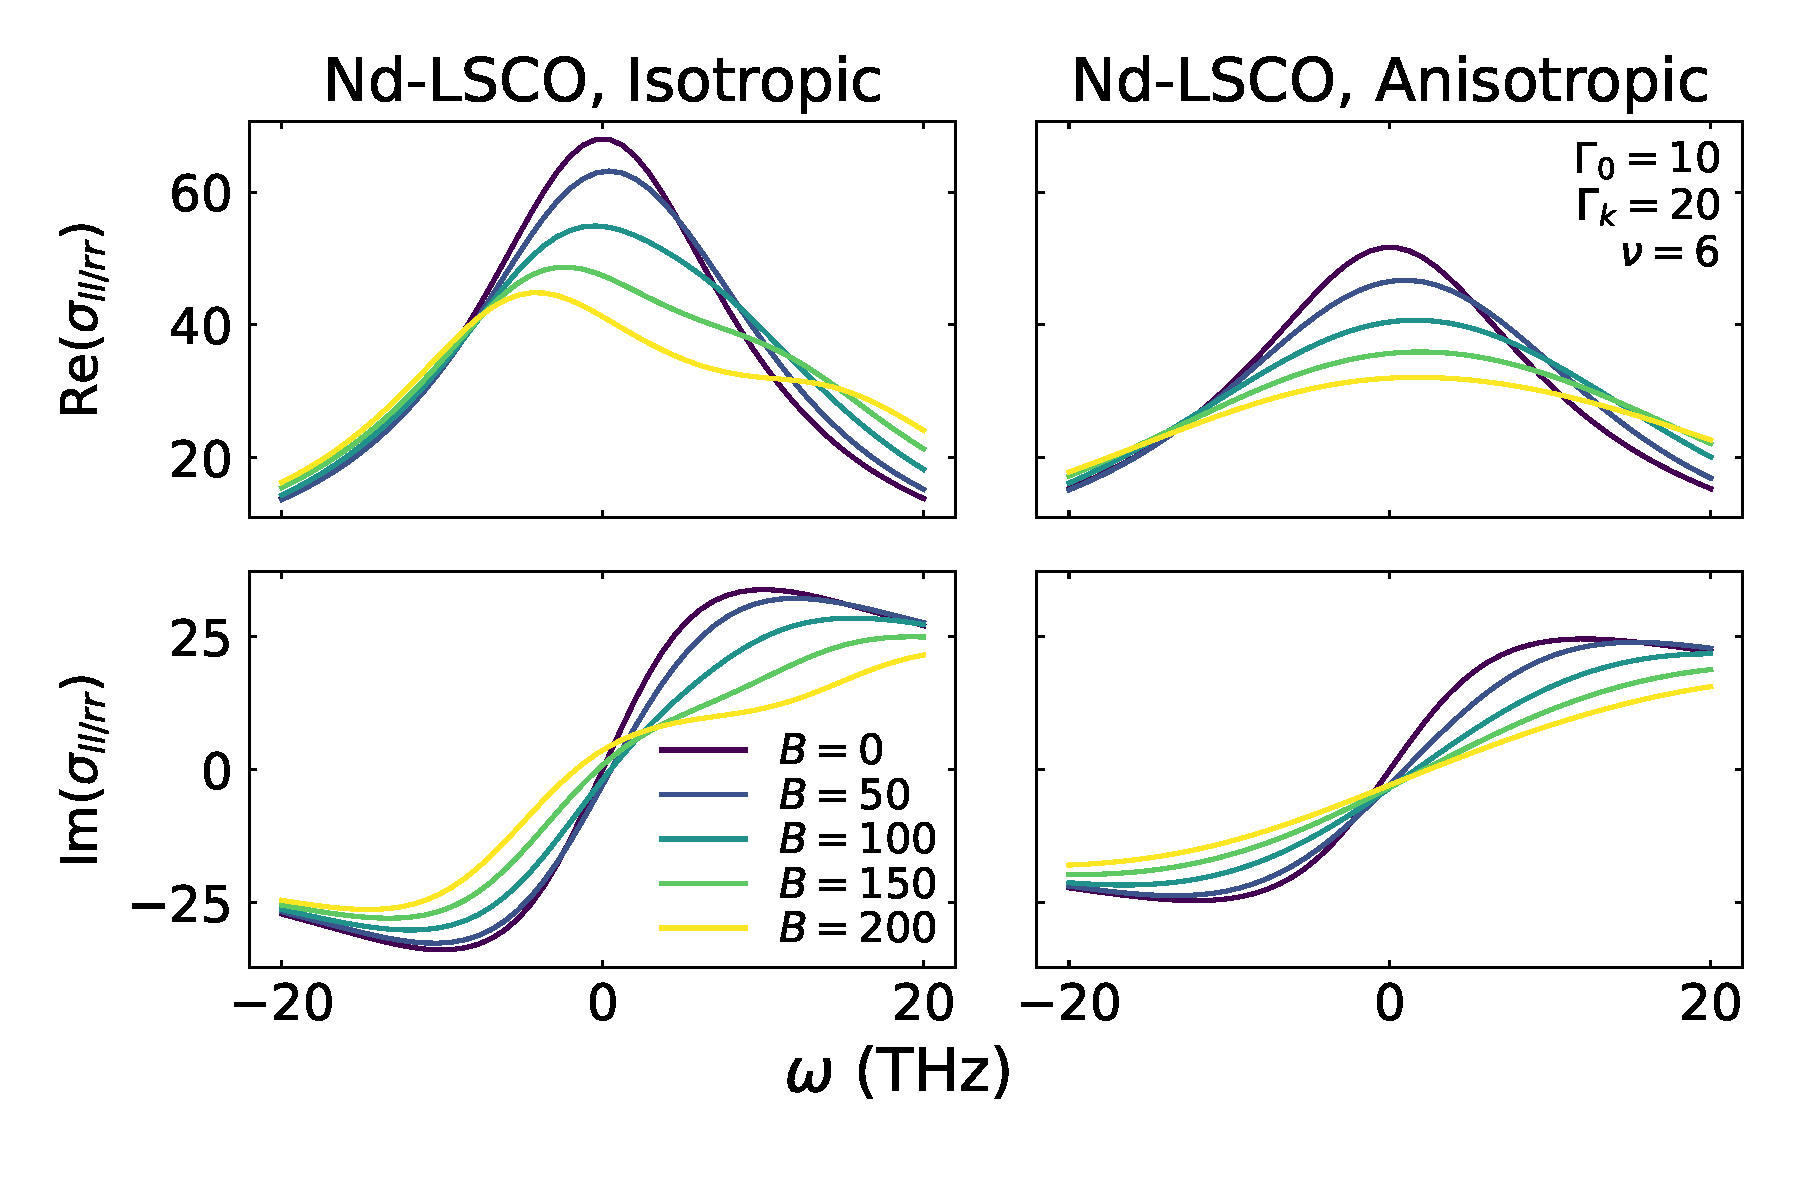
\includegraphics[width=0.7\textwidth]{figures/vary_field}
    \caption{Varying the magnetic field}
    \label{fig:vary_field}
\end{figure}


Due to the complexity of the parameter space, 
we wanted to gain a qualitative understanding of the dependence of the conductivity curve on said parameters. 
To do that, we plotted the conductivity at fixed values for all but one parameter and observed the result
(Figure \ref{fig:vary_parameters}).

Looking at the effect of the different parameters in Figure, it seems each parameter roughly has
these effects:
\begin{itemize}
    \item Isotropic scattering rate ($\Gamma_0$): affects the overall magnitude of the conductivity
        and the width of the real conductivity peak (Figure \ref{fig:vary_gamma_0}).
    \item Anisotropic scattering coefficient ($\Gamma_k$): mostly affects the magnitude of the
        conductivity (Figure \ref{fig:vary_gamma_k}).
    \item Anisotropic scattering exponent ($\nu$): affects the shape of the real conductivity peak
        and greatly affects the magnitude of the conductivity (Figure \ref{fig:vary_power}).
    \item Energy scale: affects the magnitude of the conductivity and the position of the real
        conductivity peak, which means it affects the response of the peak to the magnetic field
        (Figure \ref{fig:vary_energy_scale}).
\end{itemize}

Figure \ref{fig:vary_field} shows the exagerated effect of the magnetic field on the conductivity.
As we increase the field, we see the conductivity peak splitting into one peak going into negative
$\omega$, and another into positive $\omega$. This is due to the different effect of the magnetic
field on the two different types of charge carriers in the material: negative (electron-like)
and positive (hole-like) particles.\footnote{The Fermi surface of LSCO has electron-like
and hole-like regions} A model with no anisotropic scattering would have two conductivity peaks,
one for each type of charge carrier. The anisotropic scattering would kill one of the peaks,
because it affects electron-like particles more severely. This is because of the different
electronic properties of the material for electron-like and hole-like particles.\footnote{
The electron-like region in LSCO's Fermi surface has far more anisotropy (i.e. curvature)
than the hole-like region. See figure \ref{fig:fermi_surface}.}


\subsection{Fitting the Chambers formula to the data}
The Boltzmann transport model is way more complex than the Drude model, and can have a non-convex
optimization landscape. So we used a more sophisticated global optimization algorithm, called
differential evolution. This is a similar to a genetic algorithm, but with a few differences. It
works by creating a population of candidate solutions, and then iteratively improving them by
combining the best solutions.

The tight-binding model for the Fermi surface of LSCO has already been studied by others, so we
just used the parameters from the literature. The adjustable parameters are the scattering model
parameters and the energy scale, which is a scaling factor for the tight binding parameters,
defined as the value of $t$. The other tight binding parameters ($t'$, $t''$, and $t_z$) are
defined as multiples of $t$.

\begin{figure}
    \centering
    \begin{subfigure}{0.48\textwidth}
        \centering
        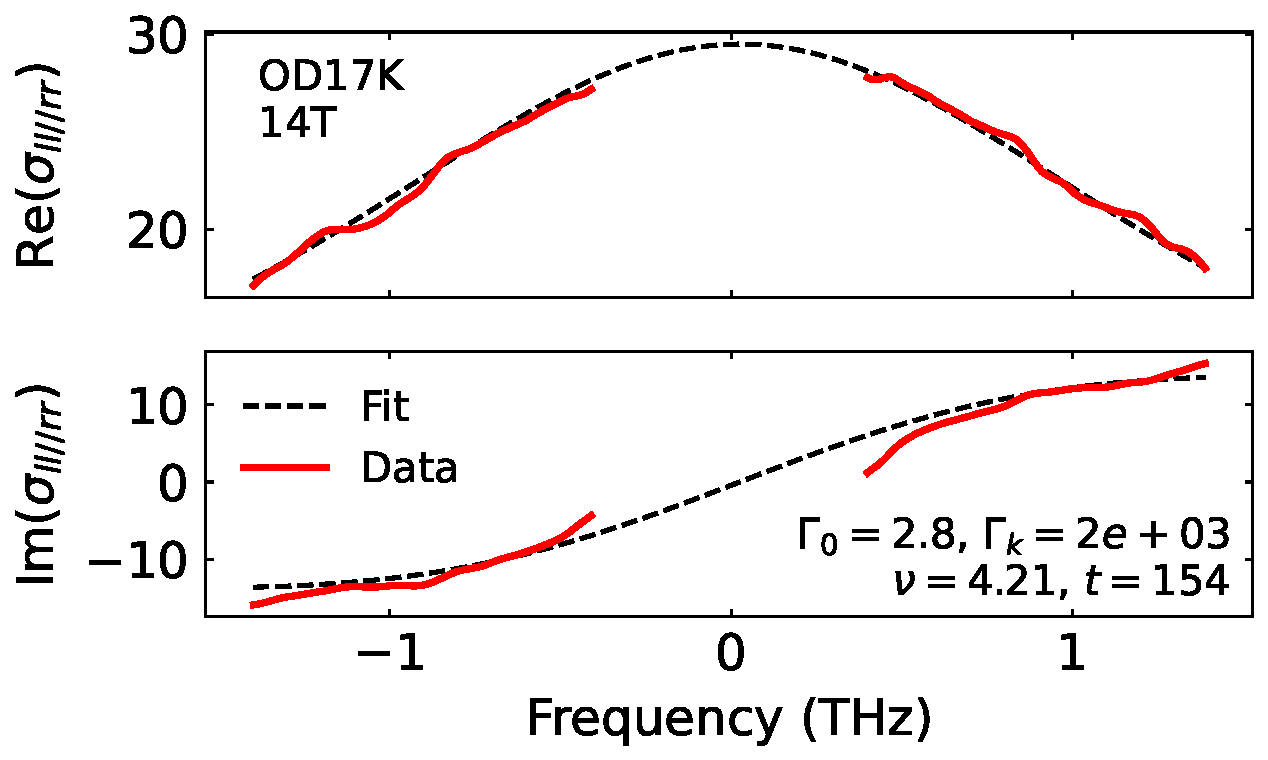
\includegraphics[width=\textwidth]{figures/fit_example_complex}
        \caption{Full complex fit}
    \end{subfigure}
    \begin{subfigure}{0.48\textwidth}
        \centering
        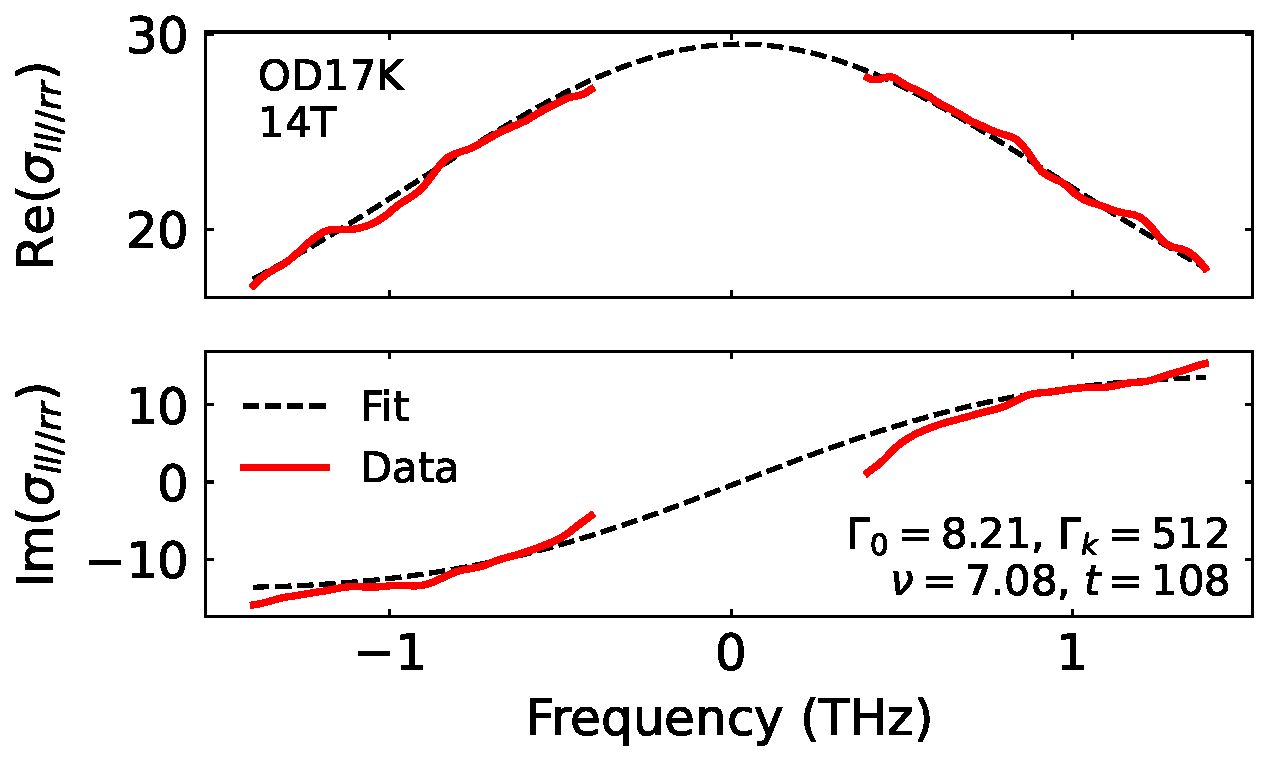
\includegraphics[width=\textwidth]{figures/fit_example_real}
        \caption{Real part fit}
    \end{subfigure}
    \caption{An example of a fit to the data. (a) shows a fit using the full conductivity data,
        while (b) shows a fit using only the real part of the conductivity. As you can see, both
        approaches do a fine job of fitting the data. Another thing to note in these plots is the
        large error and noise, especially in the imaginary part of the conductivity. The ``wrong''
        curving direction in low frequencies in the imaginary part is only present in some of the
        data, and the source is not physical.}
    \label{fig:fitting_example}
\end{figure}

Since the data is noisy and does not exhibit complex behavior, the fitting optimization problem is
very challenging. We have data for different doping levels and different magnetic fields, so a
naïve approach would be to fit the data for each doping level and each magnetic field separately.
However, fitting only to one curve at a time would not constrain the parameters enough and would
lead to many different combinations of parameters fitting the data well (Figure). So, we fit multiple
magnetic fields for each doping level simultaneously to constrain the parameters better. To make
sure our fit makes sense, we redo the fit for different sets of magnetic fields and compare the
fitting parameters. If they are consistent, we can be confident in the results.

Even with all that, the problem of an ill-posed optimization problem remains. By carefully
inspecting the fitting tendencies, we found out that this is due to the fact that the imaginary
part of the measured optical conductivity has large errors. This causes the fitting algorithm to
try to ``kill'' any features in the curve, which leads to arbitrarily large values for the
anisotropic scattering parameters. To mitigate this, we only fitted the real part of the optical
conductivity. Doing this, we can see that eventhough we have ignored the imaginary part, it will
also be fitted well, without exploding the fit parameters. This is similar to what we believe
Legros et al. did for their own fits.

\begin{figure}
    \centering
    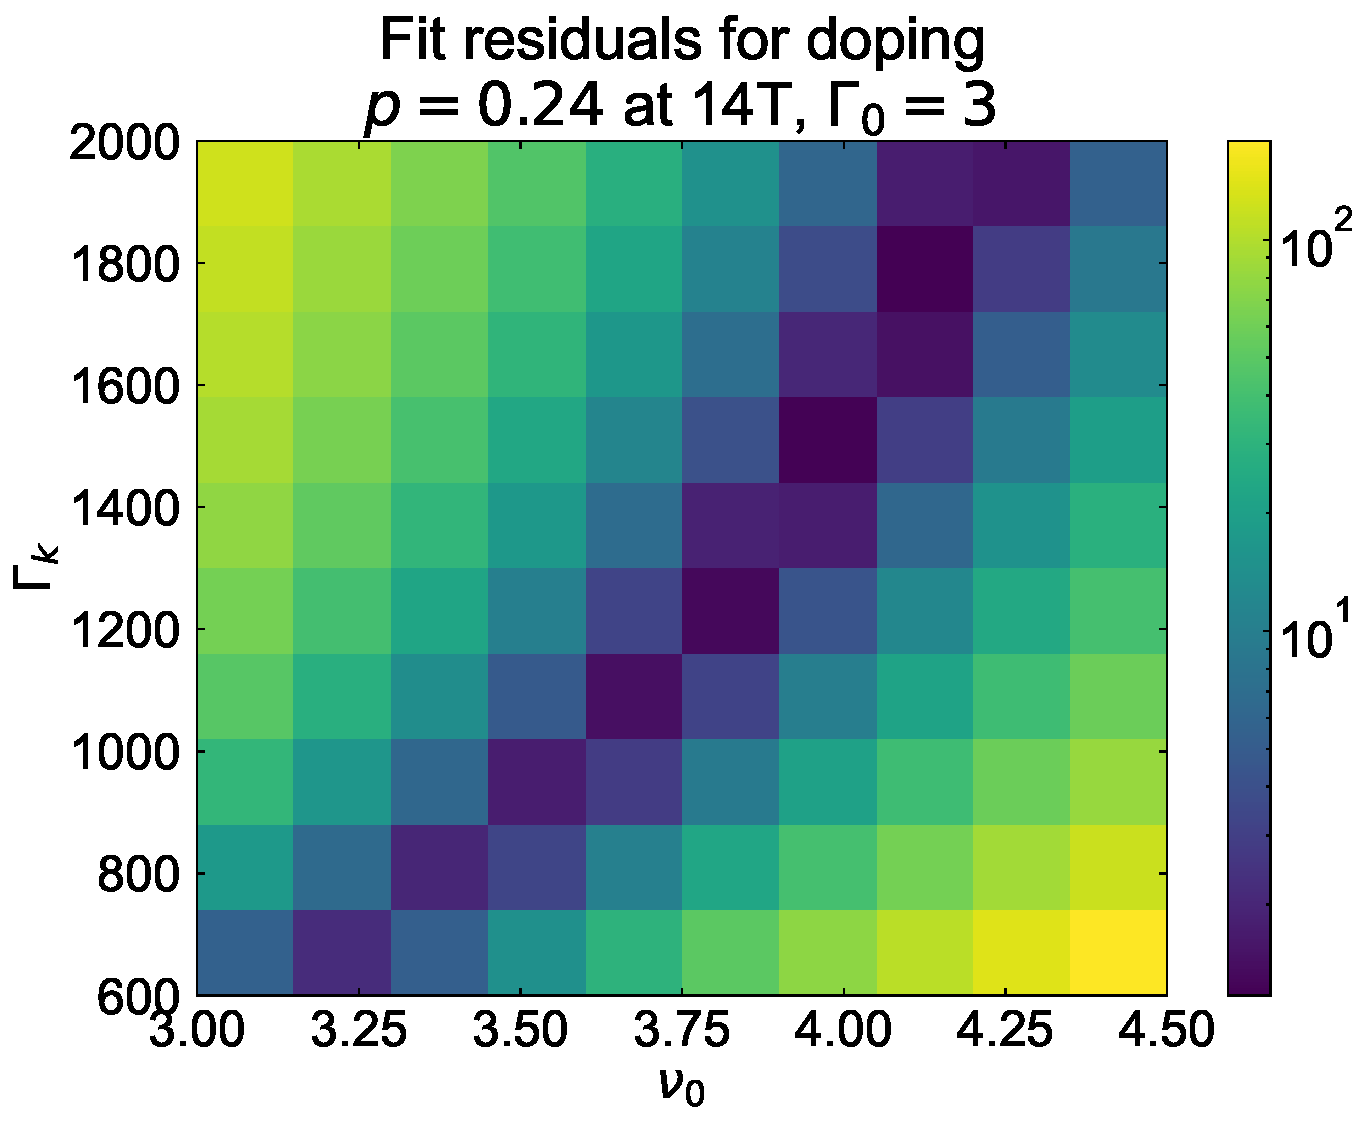
\includegraphics[width=0.5\textwidth]{figures/residuals_degenerate}
    \caption{The extremely degenerate nature of the fitting problem. This plot shows how many pairs
        of values for $\Gamma_k$ and $\nu$ make a good fit for the data.}
    \label{fig:residuals_degenerate}
\end{figure}

\subsection{Cyclotron mass}
To extract the cyclotron mass from the Chambers model, we need a new approach. In contrast to the
Drude model, here we do not have the cyclotron frequency as an explicit parameter of the formula.
We cannot use the effective mass from the dispersion relation of the tight-binding model either;
It is equal to
\begin{equation}
    m^* = \hbar^2\qty(\pdv[2]{\varepsilon}{k})^{-1}
\end{equation}
and varies for different parts of the dispersion relation. In order to define a useful parameter,
we need to average over the wavevectors. So
\begin{equation}
    m_c = \frac{\hbar}{2\pi}\oint\frac{\dd{k}}{v_\perp (k)}
\end{equation}
where $v_\perp$ is the velocity perpendicular to the magnetic field, on the path the charge
carriers take\footnote{This is a closed path on the Fermi surface, since the magnetic field does
not do work and the free charges are on the Fermi surface. The path is closed due to the periodic
nature of the oscillations.}
\newpage
\section{Conclusions \& Future Work}
Throughout this project, we adapted cutting-edge techniques for the study of cuprates to analyze
new optical conductivity data and did a thorough comparison with the older, more basic techniques.
However, due to the lack of data and the low quality of the existing data, we are unable to draw
strong conclusions yet. With more time, we could use other techniques to try to better constrain
the parameters and make better-guided fits to the data.

The optical conductivity data from Legros et al. covers a very small range of frequencies, which
makes it difficult to extract the more intricate details of the shape of the data. The big errors
and noise in some of the data points also make it difficult to find a fit that best describes the
physics of the system.

Despite all this, we believe our results contrast that of Legros et al. enough to put their data
analysis into question. Our data also follows the general trend from Michon et al. more closely,
even if it is not definitive due to the large quantitative errors and the sparsity of the data.

Future work should focus on improving the quality of the data. Increasing the range of frequencies
for measuring the optical conductivity would make huge improvements. Reducing the noise and
systematic errors in the data would also be beneficial. Finally, more data points from more
doping levels allows for a better understanding of the trends in the data. Though there is already
data available for more doping levels, which we could not use because of a lack of availablity, and
the fact that most of it is in a doping range where our analysis breaks down and a more complex
model is needed. The explanation is beyond the scope of this report, but briefly, it is because the
Fermi surface and conductive properties of cuprates are very different in the lower doping levels,
and it is not very well understood. It is still a subject of active research.
\newpage

\bibliographystyle{plain}
\bibliography{ref}

\appendix
\section{Derivation of the Chambers Formula for Optical Conductivity}
\label{sec:chambers}
Starting from the Boltzmann transport equation, if we define our density function as
$f(\vb{r}, \vb{k}; t)$ we have
\begin{equation}
    \pdv{f}{t} + \dot{\vb{k}}\vdot\grad_{\vb{k}}{f} + \dot{\vb{r}}\vdot\grad_{\vb{r}}{f}
    = \qty(\pdv{f}{t})_{\text{coll}}.
\end{equation}
In the relaxation time approximation, we have
\begin{equation}
    \qty(\pdv{f}{t})_{\text{coll}}
    = \frac{f_0(\varepsilon_{\vb{k}}) - f(\vb{r}, \vb{k};t)}{\tau(\vb{k})},
\end{equation}
where
\begin{equation}
    f_0(\varepsilon_{\vb{k}}) = \frac{1}{\exp(\beta(\varepsilon_{\vb{k}} - \mu)) + 1}
\end{equation}
is the equilibrium (Fermi-Dirac) distribution function. If we assume spatial uniformity
(which is the case when we have uniform fields over our samples), using movement equations,
we can then write
\begin{equation}
    \pdv{f}{t} - \frac{e}{\hbar}\qty(\vb{E} + \vb{v}(\vb{k})\cross\vb{B})\vdot\grad_{\vb{k}}{f}
    = \frac{f_0(\varepsilon_{\vb{k}}) - f(\vb{k};t)}{\tau(\vb{k})}.
\end{equation}
It is more useful to solve for a perturbation in the distribution $g$, such that
\begin{equation}
    f(\vb{k}; t) = f_0(\varepsilon_{\vb{k}}) + g(\vb{k}; t).
\end{equation}
Using
\begin{equation}
    \vb{v}(\vb{k}) = \frac{1}{\hbar}\grad_{\vb{k}}{\varepsilon_{\vb{k}}}
\end{equation}
and rearranging some terms, we get
\begin{equation}
    \qty(\pdv{t} + \frac{1}{\tau(\vb{k})}
    - \frac{e}{\hbar}[\vb{E}+\vb{v}(\vb{k})\cross\vb{B}]\vdot\grad_{\vb{k}})
    g(\vb{k}; t) = \frac{e\vb{E}}{\hbar}\vdot\vb{v}(k)\dv{f_0}{\varepsilon_{\vb{k}}}.
\end{equation}
Since we are only interested in the first order linear response to the electric field, we can
drop the $\vb{E}$ term on the left hand side. Also, to calculate the optical conductivity as
a function of frequency $\omega$, we apply a Fourier transform $t\to\omega$, which gives us
\begin{equation}
    \qty(-i\omega + \frac{1}{\tau(\vb{k})}
    - \frac{e}{\hbar}[\vb{v}(\vb{k})\cross\vb{B}]\vdot\grad_{\vb{k}})
    g(\vb{k}; \omega) = \frac{e\vb{E}}{\hbar}\vdot\vb{v}(\vb{k})\dv{f_0}{\varepsilon_{\vb{k}}}.
\end{equation}
Now, we plug in the cyclotron equation of motion
\begin{equation}
    \dv{k}{s} = -\frac{e}{\hbar}\vb{v}(\vb{k})\cross\vb{B}
\end{equation}
and parametrize the path $\vb{k}(s)$ with $s$ (which can be equal to time).
\begin{equation}
    \qty(-i\omega + \frac{1}{\tau(\vb{k})} + \dv{s})g(\vb{k}; \omega)
    = \frac{e\vb{E}}{\hbar}\vdot\vb{v}(\vb{k})\dv{f_0}{\varepsilon_{\vb{k}}}
\end{equation}
Integrating, we get
\begin{equation}
    g(\vb{k(s_0)}; \omega) = \dv{f_0}{\varepsilon_{\vb{k}}}e\vb{E}\vdot\int_{-\infty}^{s_0}
    \dd{s}\vb{v}(\vb{k}(s))\exp{i\omega(s_0 - s) - \int_s^{s_0}\frac{\dd{s'}}{\tau(\vb{k}(s'))}}.
\end{equation}
Using the fact that the orbit is periodic, we can just set $s_0$ to zero.

The current density is given by
\begin{equation}
    \vb{J} = -e\int\frac{\dd{\vb{k}}}{(2\pi)^d}\vb{v}(\vb{k})g(\vb{k}; \omega),
\end{equation}
where $d$ is the dimensionality of the system (the equilibtrium current vanishes).
Defining the conductivity tensor,
\begin{equation}
    \sigma_{ab} = \frac{J_a}{E_b} = -e\int\frac{\dd{\vb{k}}}{(2\pi)^d}
    v_a(\vb{k})\pdv{g(\vb{k}; \omega)}{E_b(\vb{\omega})}.
\end{equation}
Inserting the expression for $g$ and flipping the bounds of the integrals (to get a more
straightforward calculation), we get
\begin{equation}
    \sigma_{ab} = -\frac{e^2}{(2\pi)^d}\int\dd{\vb{k}}\qty(-\dd{f_0}{\varepsilon_{\vb{k}}})
    \int_0^\infty\dd{s}v_a(\vb{k})v_b(\vb{k}(s))\dv{f_0}{\varepsilon_{\vb{k}}}
    \exp{i\omega s - \int_0^s\frac{\dd{s'}}{\tau(\vb{k}(s'))}}.
\end{equation}
This is the full form of the Chambers formula. However, in normal experimental conditions,
the temperature is much lower than the Fermi temperature, so we can approximate the Fermi-Dirac
distribution as a step function. This means that the integral over the wavevectors can be reduced
to an integral over the Fermi surface. Defining $\hat{v}_a\equiv v_a/v$, we finally get the formula
used in our analysis:
\begin{equation}
    \sigma_{ab} = -\frac{e^2}{(2\pi)^d}\int_{\mathrm{FS}}\dd{\vb{k}}
    \int_0^\infty\dd{s}\hat{v}_a(\vb{k})v_b(\vb{k}(s))\dv{f_0}{\varepsilon_{\vb{k}}}
    \exp{i\omega s - \int_0^s\frac{\dd{s'}}{\tau(\vb{k}(s'))}}
\end{equation}

\section{Mathematical Equivalence of Drude and Chambers for Free Electrons}
\label{sec:equivalence}
For free electrons, the first order path is a helix with $\phi(s) = \phi(0) - \omega_c s$
where $\phi$ is the azimuthal angle. Also, we are considering a free electron dispersion, it is
isotropic in $\vb{k}$-space:
\begin{itemize}
	\item We have the energy dispersion: $E(k) = \ddfrac{\hbar^2k^2}{2m^*}$
	\item The Fermi surface is a sphere of radius $k_F$ with $\vb{k} = k_F\vu{e}_r$
	\item On the FS, $\vb{v}_F = \ddfrac{1}{\hbar}\ddfrac{\partial E(\vb{k})}{\partial\vb{k}} = \ddfrac{1}{\hbar}\ddfrac{\hbar^2}{2m^*}2k_F\vu{e}_r = \ddfrac{\hbar}{m^*}k_F\vu{e}_r$
\end{itemize} 
Now, we apply the Chambers formula:
\begin{align}
	\sigma_{xx}^{\text{Chambers}} &= \frac{2e^2}{\hbar(2\pi)^3}\displaystyle\int_{\vb{k}}^{FS}\mathop{d\vb{k}}\int_0^{\infty}\mathop{ds}
		\hat{v}_x(\vb{k})v_x(\vb{k}(s))
		\exp{-i\omega s - \int_0^s \frac{\mathop{ds'}}{\tau \vb{k}(s')}} \\
	&= \frac{e^2}{4\hbar\pi^3}\displaystyle\int_{\vb{k}}^{FS}\mathop{d\vb{k}}\int_0^{\infty}\mathop{ds}
	\hat{v}_x(\vb{k})v_x(\vb{k}(s))
		e^{(i\omega - \Gamma)s} \\
	&= \frac{e^2}{4\hbar\pi^3}\displaystyle\int_{\vb{k}, k = k_F}^{}\mathop{d\vb{k}} \hat{v}_x(\vb{k}) 
		\int_0^{\infty}\mathop{ds} v_x(\vb{k}(s)) e^{(i\omega - \Gamma)s} \\
	&= \begin{aligned}[t] \frac{e^2}{4\hbar\pi^3}&\left(\displaystyle\int_{\phi = 0}^{2\pi}\int_{\theta = 0}^{\pi}\ k_F^2\sin{\theta}\mathop{d\phi}\mathop{d\theta}(\vu{e}_r(\theta, \phi)\cdot \vu{e}_x)\right. \\
		&\left.\int_0^{\infty}\mathop{ds} v_F (\vu{e}_r(\theta(s), \phi(s))\cdot \vu{e}_x) e^{(i\omega - \Gamma)s}\right) \end{aligned} \\
	&= \begin{aligned}[t] \frac{e^2}{4\hbar\pi^3}k_F^2v_F&\left(\displaystyle\int_{\phi = 0}^{2\pi}\int_{\theta = 0}^{\pi}\ \sin{\theta}\mathop{d\phi}\mathop{d\theta} \sin{\theta}\cos{\phi} \right. \\
		&\left.\int_0^{\infty}\mathop{ds} e^{(i\omega - \Gamma)s} \sin{\theta(s)}\cos{\phi(s)}\right) \end{aligned} \\
	&= \begin{aligned}[t] \frac{e^2}{4\hbar\pi^3}k_F^2v_F&\left(\displaystyle\int_{\phi = 0}^{2\pi}\int_{\theta = 0}^{\pi} \mathop{d\phi}\mathop{d\theta} \sin^3{\theta}\cos{\phi} \right. \\
		&\left.\int_0^{\infty}\mathop{ds} e^{(i\omega - \Gamma)s} \cos{(\phi - \omega_c s)}\right) \end{aligned} \\
	&\myeq\ \frac{e^2}{4\hbar\pi^3}k_F^2v_F\displaystyle\int_{\phi = 0}^{2\pi}\int_{\theta = 0}^{\pi} \mathop{d\phi}\mathop{d\theta} \sin^3{\theta}\frac{(\Gamma - i\omega)\cos^2{\phi}+\omega_c\cos\phi\sin\phi}{(\Gamma - i\omega)^2 + \omega_c^2} \\
	&= \frac{k_F^2v_Fe^2}{4\hbar\pi^3}\frac{\frac{4}{3}\pi(\Gamma - i\omega) + 0}{(\Gamma - i\omega)^2 + \omega_c^2} = \frac{k_F^2v_Fe^2}{3\hbar\pi^2}\frac{\Gamma - i\omega}{(\Gamma - i\omega)^2 + \omega_c^2}
\end{align}
Next, substituting $v_F$ in terms of $k_F$, we get
\begin{equation}
	\sigma_{xx}^{\text{Chambers}} = \frac{k_F^3e^2}{3\pi^2m^*}\frac{\Gamma - i\omega}{(\Gamma - i\omega)^2 + \omega_c^2}.
\end{equation}
Finally, $k_F = \qty(3\pi^2n)^{1/3}$ in 3D, so it gives
\begin{equation}
    \sigma_{xx}^{\text{Chambers}} = \frac{n e^2}{3m^*}\frac{\Gamma - i\omega}{(\Gamma - i\omega)^2 + \omega_c^2}.
\end{equation}

The derivation for the off-diagonal component is similar:
\begin{align}
	\sigma_{xy}^{\text{Chambers}} &= \frac{e^2}{4\pi^3}\displaystyle\int_{\vb{k}, k = k_F}^{}\mathop{d\vb{k}} \hat{v}_x(\vb{k}) 
		\int_0^{\infty}\mathop{ds} v_y(\vb{k}(s)) e^{(i\omega - \Gamma)s} \\
	&= \begin{aligned}[t] \frac{\hbar^2 e^2}{4\pi^3}&\left(\displaystyle\int_{\phi = 0}^{2\pi}\int_{\theta = 0}^{\pi}\ k_F^2\sin{\theta}\mathop{d\phi}\mathop{d\theta}(\vu{e}_r(\theta, \phi)\cdot \vu{e}_x)\right. \\
		&\left.\int_0^{\infty}\mathop{ds} v_F (\vu{e}_r(\theta(s), \phi(s))\cdot \vu{e}_y) e^{(i\omega - \Gamma)s}\right) \end{aligned} \\
	&= \begin{aligned}[t] \frac{\hbar^2 e^2}{4\pi^3}k_F^2v_F&\left(\displaystyle\int_{\phi = 0}^{2\pi}\int_{\theta = 0}^{\pi}\ \sin{\theta}\mathop{d\phi}\mathop{d\theta} \sin{\theta}\cos{\phi} \right. \\
		&\left.\int_0^{\infty}\mathop{ds} e^{(i\omega - \Gamma)s} \sin{\theta(s)}\sin{\phi(s)}\right) \end{aligned} \\
	&= \begin{aligned}[t] \frac{\hbar^2 e^2}{4\pi^3}k_F^2v_F&\left(\displaystyle\int_{\phi = 0}^{2\pi}\int_{\theta = 0}^{\pi} \mathop{d\phi}\mathop{d\theta} \sin^3{\theta}\cos{\phi} \right. \\
		&\left.\int_0^{\infty}\mathop{ds} e^{(i\omega - \Gamma)s} \sin{(\phi - \omega_c s)}\right) \end{aligned} \\
	&\myeq\ \frac{\hbar^2 e^2}{4\pi^3}k_F^2v_F\displaystyle\int_{\phi = 0}^{2\pi}\int_{\theta = 0}^{\pi} \mathop{d\phi}\mathop{d\theta} \sin^3{\theta}\frac{(\Gamma - i\omega)\cos{\phi}\sin\phi-\omega_c\cos^2\phi}{(\Gamma - i\omega)^2 + \omega_c^2} \\
	&= \frac{k_F^2v_Fe^2}{4\hbar\pi^3}\frac{0 - \frac{4}{3}\pi\omega_c}{(\Gamma - i\omega)^2 + \omega_c^2} = -\frac{\hbar^2 k_F^2v_Fe^2}{3\pi^2}\frac{\omega_c}{(\Gamma - i\omega)^2 + \omega_c^2}
\end{align}
\begin{equation}
	\sigma_{xy}^{\text{Chambers}} = -\frac{k_F^3e^2}{3\pi^2m^*}\frac{\omega_c}{(\Gamma - i\omega)^2 + \omega_c^2}
    = -\frac{n e^2}{3m^*}\frac{\omega_c}{(\Gamma - i\omega)^2 + \omega_c^2}
\end{equation}

After all these calculations, to convert to the circular basis for comparing to the Drude
model,\footnote{we rederived the Drude model in Cartesian basis too, it is just simpler to compare
to the circular basis already stated in the report and writing extra calculations for the Drude
model here is redundant.} we use the Kramers--Kronig relations.
\begin{align}
    \sigma_{ll/rr} &= \sigma_{xx} + i\sigma_{xy} = \frac{n e^2}{3m^*}
    \frac{\Gamma - i(\omega + \omega_c)}{(\Gamma - i\omega)^2 + \omega_c^2} \\
    &= \frac{n e^2}{3m^*}\frac{(\Gamma - i\omega) - i\omega_c}
    {[(\Gamma - i\omega) + i\omega_c][(\Gamma - i\omega) - i\omega_c]} \\
    &= \frac{n e^2}{3m^*}\frac{1}{\Gamma - i(\omega - \omega_c)} = \frac{n e^2}{3m^*}\frac{i}{\omega - \omega_c + i\Gamma}
\end{align}
When defining $\omega^2_{\mathrm{p,n}} = \frac{ne^2}{\epsilon_0 m^*}$, This is exactly the same as
the Drude formula in the circular basis, without the effect of supercunductivity.


\end{document}